\documentclass[a4paper,12pt]{report}
\usepackage[utf8]{inputenc}
\usepackage[T1]{fontenc}
\usepackage[english]{babel}
\usepackage{lmodern}

%hyperref for interactive PDF index
\usepackage[bookmarks, colorlinks, breaklinks]{hyperref}
\hypersetup{linkcolor=black, citecolor=black, filecolor=black, urlcolor=black}

%Package required to use special symbols
\usepackage{amsmath, amssymb}

%tPackage for tables
\usepackage{tabu}
\usepackage{tabularx}
\usepackage{ltablex}
\usepackage{longtable}
\usepackage{float} % To allow the use of H modifier in long tables

%Package required to use figures
\usepackage{graphicx}
%Include the bibliography in the table of contents
\usepackage{tocbibind}

%Package used to insert figures at the specified position
\usepackage{float}

%To call Chapters -> Sections
\addto\captionsenglish{\renewcommand{\chaptername}{Section}}

%To have a new line after a \paragraph
\newcommand{\myparagraph}[1]{\paragraph{#1}\mbox{}\\}

%References Packages
\usepackage{xr-hyper}
\usepackage{hyperref}

\begin{document}

%Title page
\begin{titlepage}
\centering
	\begin{center}{
		\begin{figure}[h]
		\large
		\centering
		{
\includegraphics[width=.60\linewidth]{img/logo_poli}}
        \end{figure}
    	}
	\end{center}
	\vspace{1 cm}
	{\Large {\textbf{\LARGE TrackMe} \\
		Software Engineering II - Prof. Elisabetta Di Nitto} \par}
	\vspace{1.5cm}
	{\LARGE \textbf{Design Document} \par}
	\vspace{1.5cm}
	{\Large\itshape Michele Gatti, Federica Gianotti, Mathyas Giudici\par}
	\vspace{2cm}
	\vfill
	% Bottom of the page
	{\large Document version: 1.0\par}
	{\large \today \par}
\end{titlepage}

{
\begin{table}[h!]
\begin{tabu} to \textwidth { X[0.3,r,p] X[0.7,l,p] }
\textbf{Deliverable:} & DD\\
\textbf{Title:} & Design Document \\
\textbf{Authors:} & Michele Gatti, Federica Gianotti, Mathyas Giudici \\
\textbf{Version:} & 1.0 \\
\textbf{Date:} & \today \\
\textbf{Download page:} & https://github.com/MathyasGiudici/GattiGianottiGiudici \\
\textbf{Copyright:} & Copyright © 2018, Michele Gatti, Federica Gianotti, Mathyas Giudici – All rights reserved \\
\end{tabu}
\end{table}

\setcounter{page}{2}
}

%Make the table of contents
\setcounter{tocdepth}{1}
\tableofcontents

%Introduction
\chapter{Introduction}
\section{Purpose}
The  goal of the Requirement Analysis and Specification Document (RASD) is to give a clear description of the system that is going to be developed, its functional and non-functional requirements, its constraints and its domain. Moreover, it provides information about the relationship between the system taken into account and the external world by providing use cases and scenarios. Finally it gives a more formal specification of the most relevant features of the system to be using the Alloy language.
Generally this type of document is mainly addressed to developers, programmers, testers, project managers and system analysists, but it can be useful also for final users.
Track Me is a company that wants to develop three different but connected software-based services:
\begin{itemize}
  \item \textbf{Data4Help}: a service that allows third parties to monitor the location and health status of individuals. Through this service third parties can request the access both to the data of some specific individuals, who can accept or refuse sharing their information , and to anonymized data of group of individuals, which will be given only if the number of the members of the group is higher than 1000, according to privacy rules.
  \item \textbf{AutomatedSOS}: a service addressed to elderly people which monitors the health status of the subscribed customers and, when such parameters are below a certain threshold (personalized for every user using the data from Data4Help), sends to the location of the customer an ambulance, guaranteeing a reaction time less than 5 second from the time the parameters are below the threshold.
  % \clearpage
  \item \textbf{Track4Run}: a service to track athletes participating in a run. It allows organizers to define the path for a run, participants to enroll to a run and spectators to see on a map the position of all runners during the run. This service will exploit the features offered by Data4Help.
\end{itemize}

\subsection{Goals}
The three applications of the system have in common the following goals:
\begin{itemize}
  \item \textbf{[G.1]}: Allow unregistered user to sign in to access to the application;
  \item \textbf{[G.2]}: Allow registered user to log in and access to the application;
  \item \textbf{[G.3]}: Allow registered user to manage his/her profile;
\end{itemize}

The description given above can be summarized as a list of goals, specific for each service.
\paragraph{Data4Help:}
\begin{itemize}
  \item \textbf{[G.4]}: Allow registered third parties to request data of a single individual;
  \item \textbf{[G.5]}: Allow registered third parties to request data of a group of people;
\end{itemize}

\paragraph{AutomatedSOS:}
\begin{itemize}
  \item \textbf{[G.6]}: Allow data acquisition through smart watches (or similar);
  \item \textbf{[G.7]}: Allow monitoring the health status of an individual registered user;
  \item \textbf{[G.8]}: Allow sending location of an individual registered user to an ambulance if his/her parameters are below a certain threshold;
\end{itemize}

\paragraph{Track4Run:}
\begin{itemize}
  \item \textbf{[G.9]}: Allow registered user to become organizers or athletes of a run;
  \item \textbf{[G.10]}: Allow organizers to define the date and the path for a new run;
  \item \textbf{[G.11]}: Allow organizers to delete a run;
  \item \textbf{[G.12]}: Allow registered athletes to enrol to a run;
  \item \textbf{[G.13]}: Allow registered athletes to delete an enrolment of a run;
  \item \textbf{[G.14]}: Allow unregistered user to access as spectator;
  \item \textbf{[G.15]}: Allow registered/unregistered user to see on a map the position of all runners during a run;
\end{itemize}

\section{Scope}
According to \textit{The World and the Machine} \cite{world-machine} we can divide every system into two parts:
\begin{itemize}
  \item The \textbf{machine}, which is the portion of system to be developed;
  \item The \textbf{world}, which is the portion of the real-world affected by the machine.
\end{itemize}
As a consequence we can classify phenomena in three different types:
\begin{itemize}
  \item \textbf{World phenomena}: phenomena that the machine cannot observe;
  \item \textbf{Machine phenomena}: phenomena located entirely in the machine;
  \item \textbf{Shared phenomena}: phenomena that can be controlled by the world and observed by the machine or controlled by the machine and observed by the world;
\end{itemize}
Below we give an analysis of world and shared phenomena:
\paragraph{World phenomena}
\begin{itemize}
  \item A user turns on data connection;
  \item A user wears his smartwatch during a day;
  \item The batteries of the smartwatch of a user run out;
  \item A user turns on the GPS;
  \item An enrolled runner for a run takes part in it;
  \item A runner wears his smartwach during a run.
\end{itemize}
\paragraph{Shared phenomena}
\begin{itemize}
  \item New user registeres to Data4Help service;
  \item A Data4Help registered user logs into the system;
  \item A user recives a request to share his data;
  \item A user accept/decline a request to share his data;
  \item A third party requires data of a specific user;
  \item A third party requires data of a group of users;
  \item A user subscribes to AutomatedSOS service;
  \item An ambulance is called as a consequence of specific acquired data from the system;
  \item A Data4Help user access to Track4Run for the first time;
  \item A Track4Run user organizes a new run;
  \item A Track4Run user enrols for a run;
  \item An unregistered user access as a spectator to a run.
\end{itemize}
\paragraph{Machine phenomena}
\begin{itemize}
  \item The machine interfaces with external software and hardware systems;
  \item The machine manages database queries;
  \item The machine manages the 3G/4G Internet connection;
  \item The machine manages the Bluetooth connection;
  \item The machine manages GPS tracking.
\end{itemize}

\begin{figure}[H]
\begin{center}
  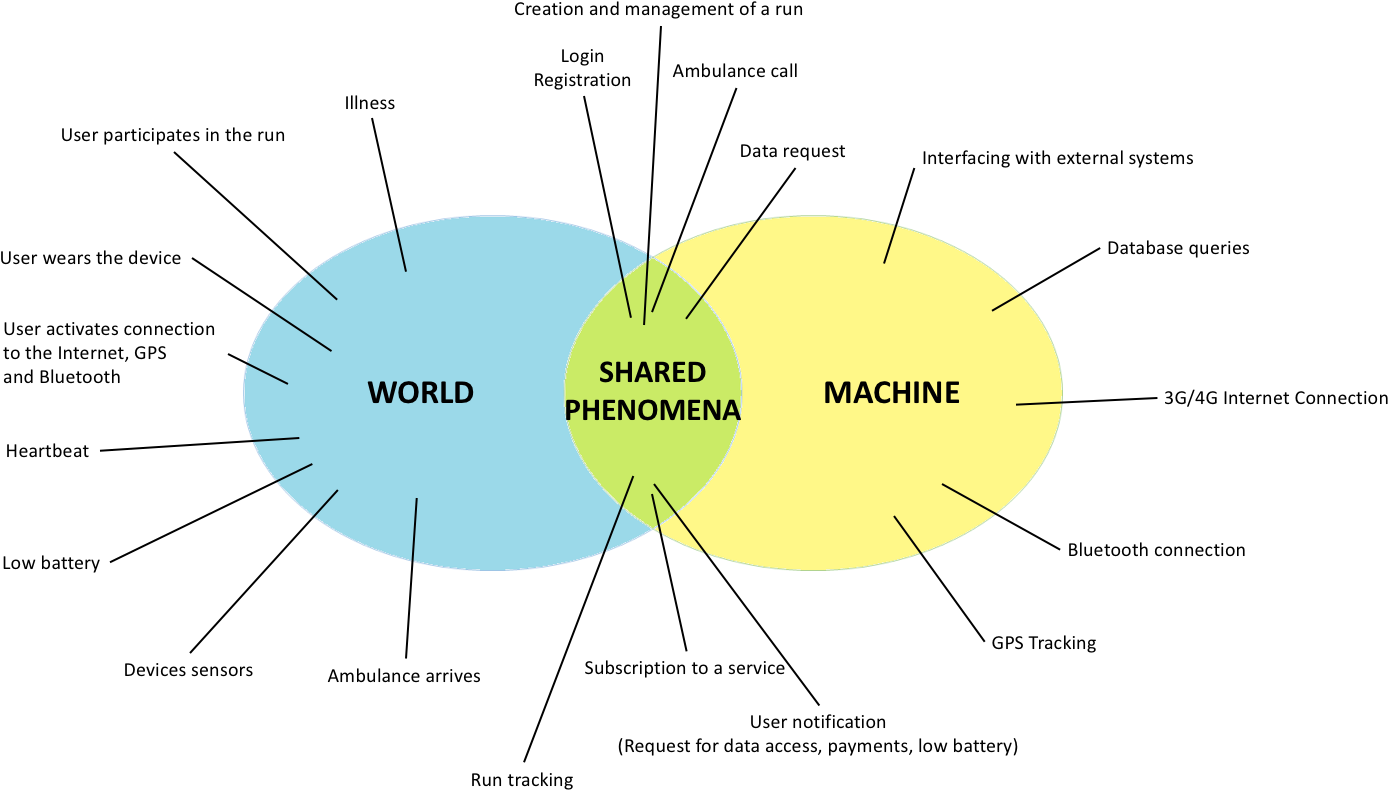
\includegraphics[width=\textwidth]{img/WorldMachine.png}
  \hspace{0.05\linewidth}
  \centering
  \caption{World and Machine model}
  \label{img:WandMmodel}
\end{center}
\end{figure}

\section{Definitions, Acronyms and Abbreviations}
\begin{itemize}
  \setlength{\itemindent}{-.4in}
  \item[] \textbf{API}: Application Programming Interface;
  \item[] \textbf{GPS}: Global Positioning System;
  \item[] \textbf{Organizer}: A registered user that organizes a run, defining date and path;
  \item[] \textbf{OS}: Operating System;
  \item[] \textbf{RASD}: Requirement Analysis and Specification Document;
  \item[] \textbf{Run}: An event that is organized by one organizer, at which one or more people can partecipate and that can be followed by one or more spectators;
  \item[] \textbf{Runner}: A registered user that enrols for a run;
  \item[] \textbf{Spectator}: Unregistered user that access to Track4Run to follow a run;
  \item[] \textbf{SSN}: Social Security Number;
  \item[] \textbf{System}: The software system-to-be, including all of its services;
  \item[] \textbf{Third party}: Any external organization that wants to access to data acquired by Data4Help;
  \item[] \textbf{UML}: Unified Modeling Language;
  \item[] \textbf{User}: Any person, registered or not, who accesses to one of the applications (for Data4Help there is a special user called \textit{Third party});
  \item[] \textbf{VAT}: Value Added Tax.
\end{itemize}

\section{Reference documents}
------------------ TODO ------------------

\section{Overview}
This document is structured as follows:
\begin{itemize}
  \setlength{\itemindent}{-.4in}
  \item[] \textbf{Section 1: Introduction}. A general introduction to the goals, the phenomena and the scope of the system-to-be. It aims giving general but exaustive information about what this document is going explain.
  \item[] \textbf{Section 2: Overall Description}.
  \item[] \textbf{Section 3: Specific Requirements}.
  \item[] \textbf{Section 4: Effort Spent}. A summary of the worked time by each member of the group.
\end{itemize}
At the end there is the bibliography.

\clearpage

%Architectural Design
\chapter{Architectural Design}
 \section{Overview}
The main high-level components of the system that will be taken into account are structured in four layers, as shown in Figure \ref{img:layeredStructure} below.

\begin{figure}[H]
  \begin{center}
  	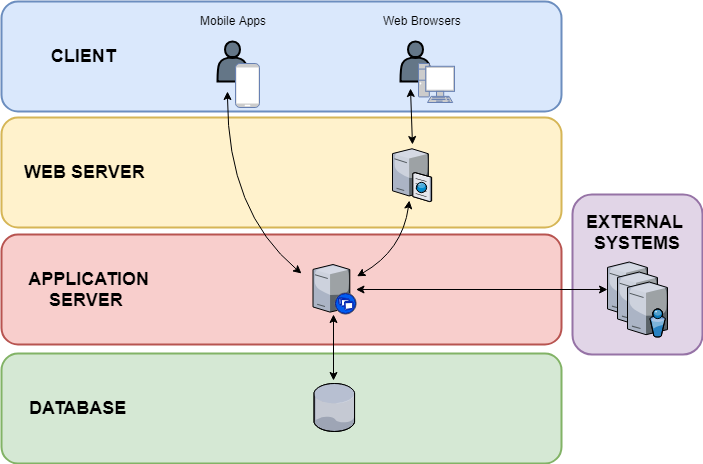
\includegraphics[width=\textwidth]{./img/LayeredStructure.png}
    \hspace{0.05\linewidth}
    \centering
    \caption{\textit{Layered Structure} of the system.}
		\label{img:layeredStructure}
    \end{center}
\end{figure}

The considered high-level components are:
\begin{itemize}
  \setlength{\itemindent}{-.4in}
  \item[] \textbf{Mobile Applications:} The \textit{Presentation Layer} dedicated to mobile devices; it communicates with the Application Server.
  \item[] \textbf{Web Browsers:} The \textit{Presentation Layer} dedicated to web browsers; it communicates directly with the Web Server.
  \item[] \textbf{Web Server:} This is the layer that provides web-pages for the web-based applications; it communicates with the Application Server and with the Web Browsers.
  \item[] \textbf{Application Server:} This is the layer in which is contained all the \textit{logic} for the application; it communicates with the Web Server and with the Database. Moreover it manages the communication with External Services.
  \item[] \textbf{Database:}  The \textit{Data Layer} of the system; it includes all structures and entities responsible for data storage and management. It communicates with the Application Server.
\end{itemize}
It has been taken the decision to separate the Application and Web Server in order to allow greater scalability. In the figure above it is also shown the interaction between the Application Server and External Systems.
A more detailed description of the intereactions between the described system components is shown in Figure \ref{img:highLevelComponents}.

\begin{figure}[H]
  \begin{center}
  	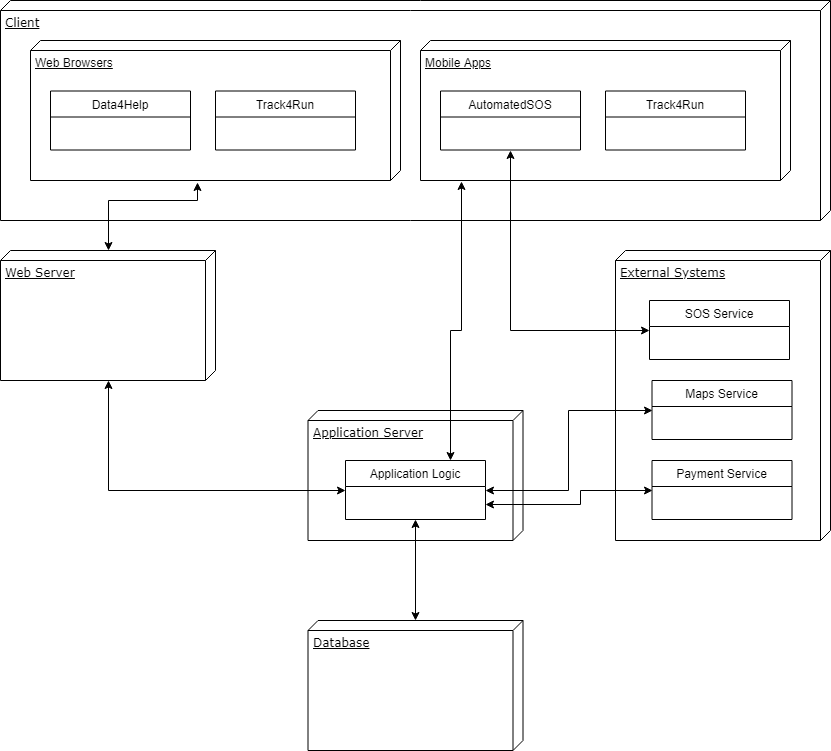
\includegraphics[width=\textwidth]{./img/HighLevelComponents.png}
    \hspace{0.05\linewidth}
    \centering
    \caption{\textit{High Level Components} of the system.}
		\label{img:highLevelComponents}
    \end{center}
\end{figure}

\section{Component View}
In this section the system will be described in term of its components. Functionalities of the components will be discussed and detailed will be shown the interfaces among components and among external services.

\subsection{Database}
The application database will be managed using a Relational DBMS.
It allows the reading of data, ensuring users the ability to log in and access the applications of interest and check the stored data.
It is also used for data manipulation (insertion, modification and deletion).
The use of a Relational DBMS guarantees the fundamental properties for a database of this type:
\begin{itemize}
  \item \textit{Atomicity}: no partial executions of operations.
  \item \textit{Consistency}: the database is always in a consistent state.
  \item \textit{Isolation}: each transaction is executed in an isolated and independent way.
  \item \textit{Durability / Persistence}: changes made are not lost.
\end{itemize}
The database will offer to the Application Server an interface that it can use to interact with the database.
The data stored in the database must be considered personal and confidential, therefore, procedures must be implemented to safeguard the stored information.\\
Particular attention must be paid to the reading permissions granted to users and to the encryption of passwords used to access the services offered.
Below is the designed E-R diagram.(Figure \ref{img:ER_Diagram})

\begin{figure}[H]
  \begin{center}
  	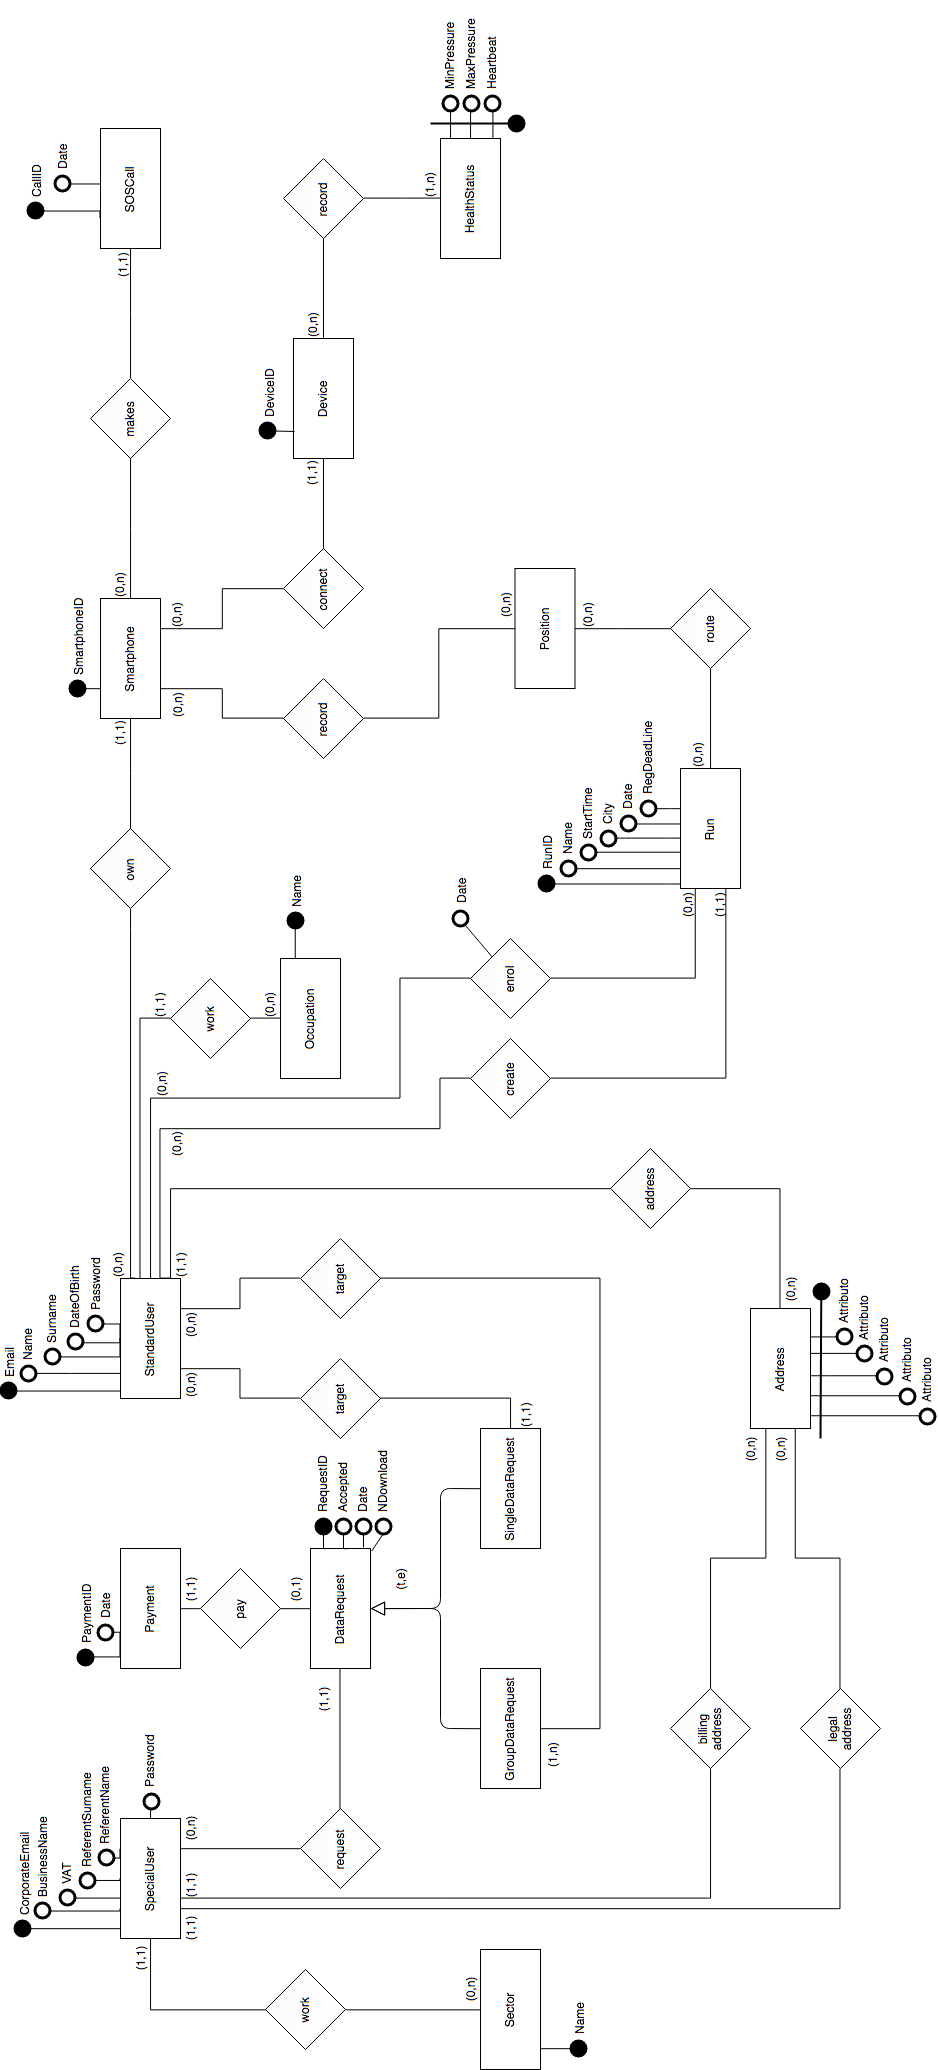
\includegraphics[height=0.68\paperheight]{./img/ER.png}
    \hspace{0.05\linewidth}
    \centering
    \caption{\textit{E-R} Diagram}
		\label{img:ER_Diagram}
    \end{center}
\end{figure}

\subsection{Application Server}
This is the crucial layer of the system to be. The main feature of the \textit{Application Server} is to describe rules and work-flows of all the functionalities provided by the application.\\
The \textit{Application Server} must have intefaces to communicate with the \textit{Web Server} and the \textit{Mobile Apps}, it has also to communicate through interfaces with all the \textit{External Services} (Maps Service, SOS Service and Payment Service).\\
Moreover, the \textit{Application Server} is the only entity of the system that is granted to communicate with the DBMS.
Following this brief introduction there are the logic modules and their descriptions, moreover all connections among components could be seen in the \textit{Global Component View} in Figure \ref{img:GlobalComponent}.

\paragraph{Data Collector Service}
This module offers the a service to the \textit{Standard User Manager} in order to maange user's data and store it into the \textit{Data4Help} database.

\paragraph{Group Request Manager}
This module manages the third party requests of \textit{Group Data Requirement}.

\paragraph{Mail Manager}
This module is a tool for other modules that allow the system to send e-mail, for instance in the registration and enrolment phase.

\paragraph{Maps Manager}
This module is an handler providing an interface to the external service of maps.

\paragraph{Payment Handler}
This module is an handler providing an interface to the external service of payment.

\paragraph{Persistence Unit}
This module is the unique interface to the database's DBMS.

\paragraph{Run Manager}
This module manages \textit{Runs} in all their functionalities, like creation, deletion and enrolment.\\
In order to manage guest users that visit a Run the system this module provides an access point to the \textit{Application Server} for the \textit{Web Server} and the \textit{Mobile Apps}.

\paragraph{Single Request Manager}
This module manages the third party requests of \textit{Single Data Requirement}.

\paragraph{Special User Manager}
This module provides all functionalities related to the \textit{Special User}.

\paragraph{Standard User Manager}
This module provides all functionalities related to the \textit{Standard User}.


\subsection{Mobile App}
The \textit{Mobile App} must communicate to the \textit{Application Server} through APIs that have to be defined in order to describe the interactions between the two layers and they must be indipendent from the implementation both side.\\
The App UI must be designed user friendly and it has to follow the guidelines provided by the Android and iOS producer.
The application must provide a software module that manages the GPS connection of the device and keeps track of locations data, it has also to manage the Health data from the devices connected to the phone.\\
The application must provide all collected data to the \textit{Application Server} in order to process them.

\subsection{AutomatedSOS App}
In this Section we want to specify in detail the modules that compose the \textit{AutomatedSOS} application in order to better explain the important activity of detection of possible \textit{Critical Situation}.\\
All connections among components could be seen in the \textit{AutomatedSOS Component View} in Figure \ref{img:AutomatedComponent}.

\paragraph{Application Server Handler}
This module is an handler providing an interface to the \textit{Application Server}.

\paragraph{Background Health Monitor}
This module checks status of health data that it receives. If an SOS call must be done it call \textit{SOS Handler}.

\paragraph{GUI}
This module is the \textit{Graphical} interface to the smartphone.

\paragraph{Health Status Service}
This module manage data detected and produce statistic for the \textit{User}.

\paragraph{SOS Handler}
This module is an handler providing an interface to the external service of SOS.

\subsection{Web Server}
The \textit{Web Server} must communicate to the \textit{Application Server} through HTTPS protocol.\\
The \textit{GUI} of the \textit{}{Web Server} must be designed user friendly and it has to follow the guidelines provided by W3C standard (using HTML5, CSS and JS).\\
The \textit{Control Unit} manages all actions played by a user and it must communicate to the \textit{Application Server} through APIs, that are already explained for the \textit{Mobile App}.

\begin{figure}[H]
  \begin{center}
  	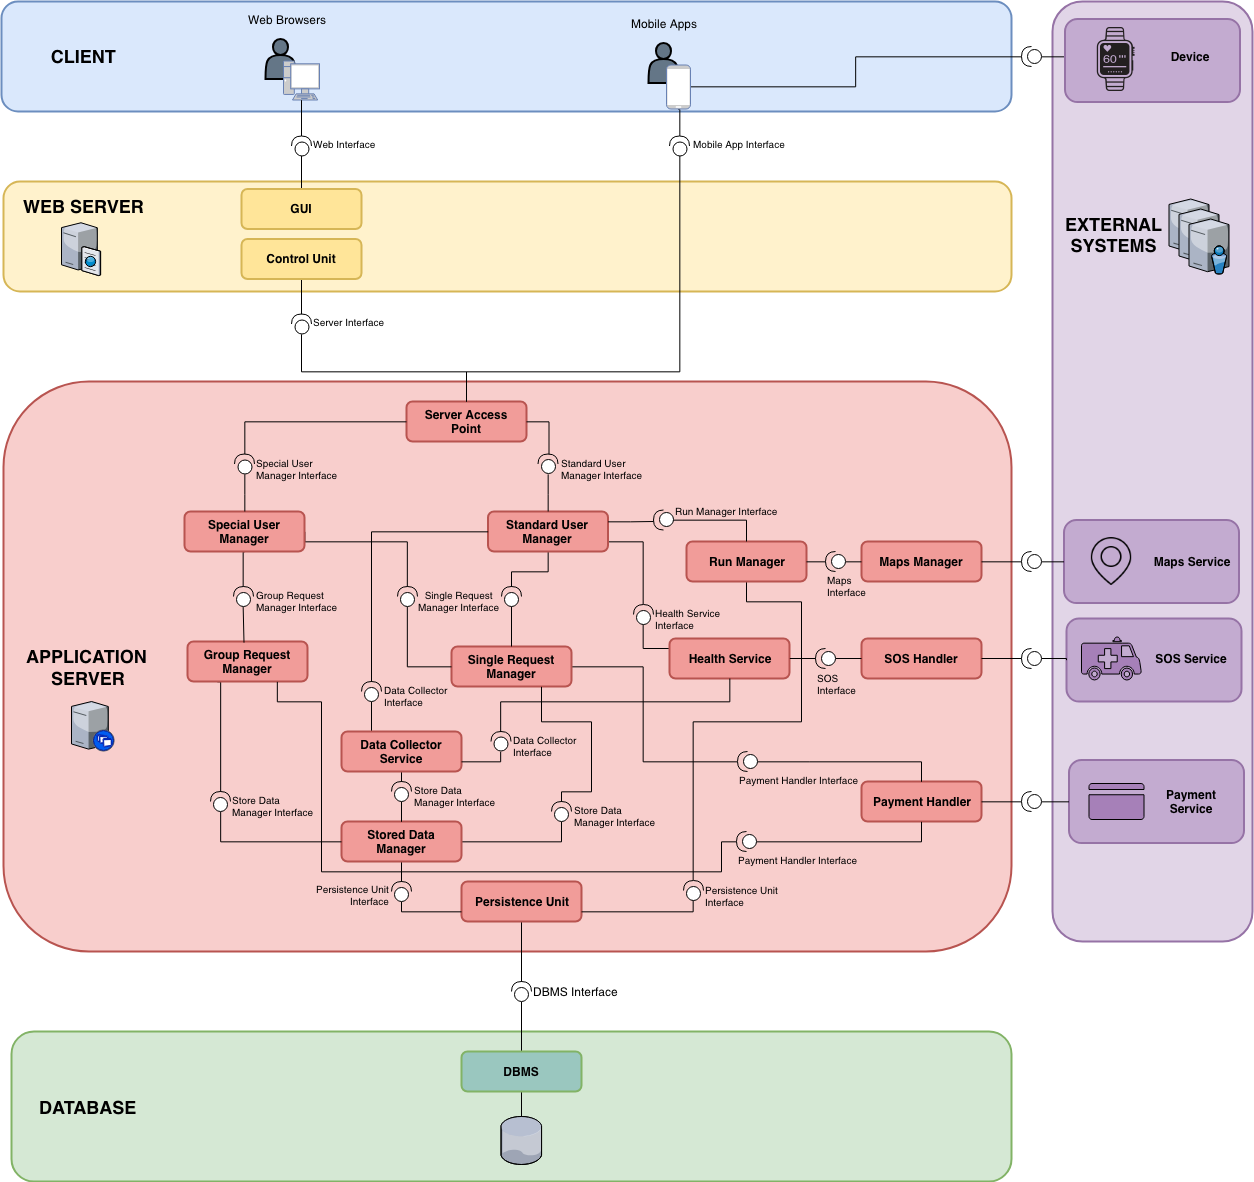
\includegraphics[width=\textwidth]{./img/GlobalComponent.png}
    \hspace{0.05\linewidth}
    \centering
    \caption{\textit{Global Component View}}
		\label{img:GlobalComponent}
    \end{center}
\end{figure}

\begin{figure}[H]
  \begin{center}
  	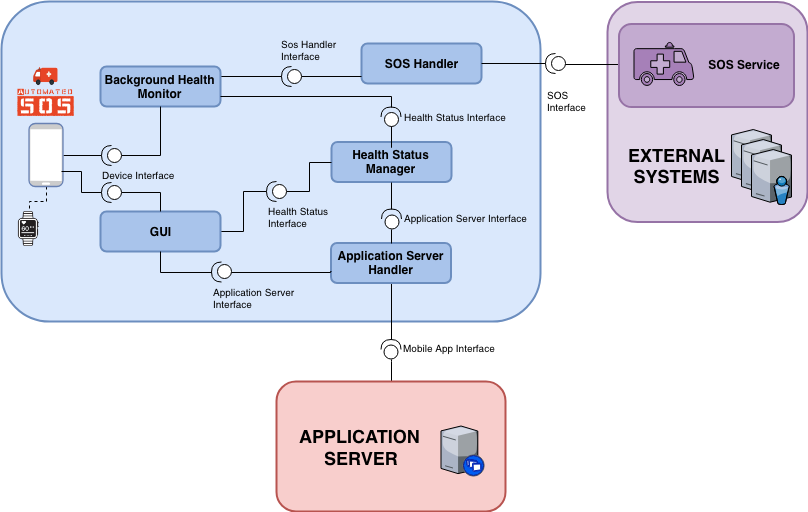
\includegraphics[width=\textwidth]{./img/Automated_Component.png}
    \hspace{0.05\linewidth}
    \centering
    \caption{\textit{AutomatedSOS Component View}}
		\label{img:AutomatedComponent}
    \end{center}
\end{figure}

\clearpage

\section{Deployment View}
Below is the deployment diagram of the system to be (Figure \ref{img:Deployment_Diagram}).

\begin{figure}[H]
  \begin{center}
  	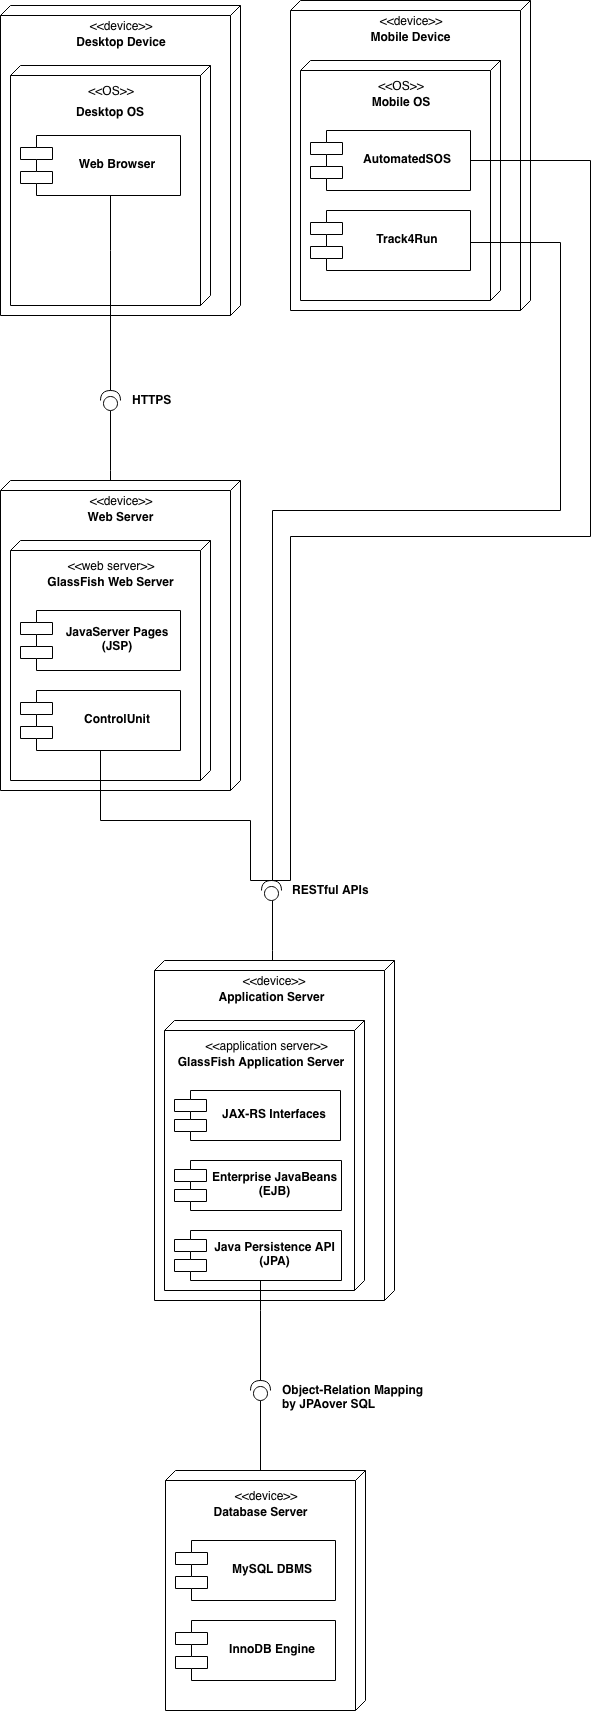
\includegraphics[height=0.59\paperheight]{./img/Deployment_Diagram.png}
    \hspace{0.05\linewidth}
    \centering
    \caption{Deployment Diagram of the system to be}
		\label{img:Deployment_Diagram}
    \end{center}
\end{figure}

\clearpage

\section{Runtime View}\label{runtimeViewSection}
In this Section we want to specify the behaviour of our system. Some relevant cases are selected and explained using Sequence Diagrams.

\begin{figure}[H]
  \begin{center}
  	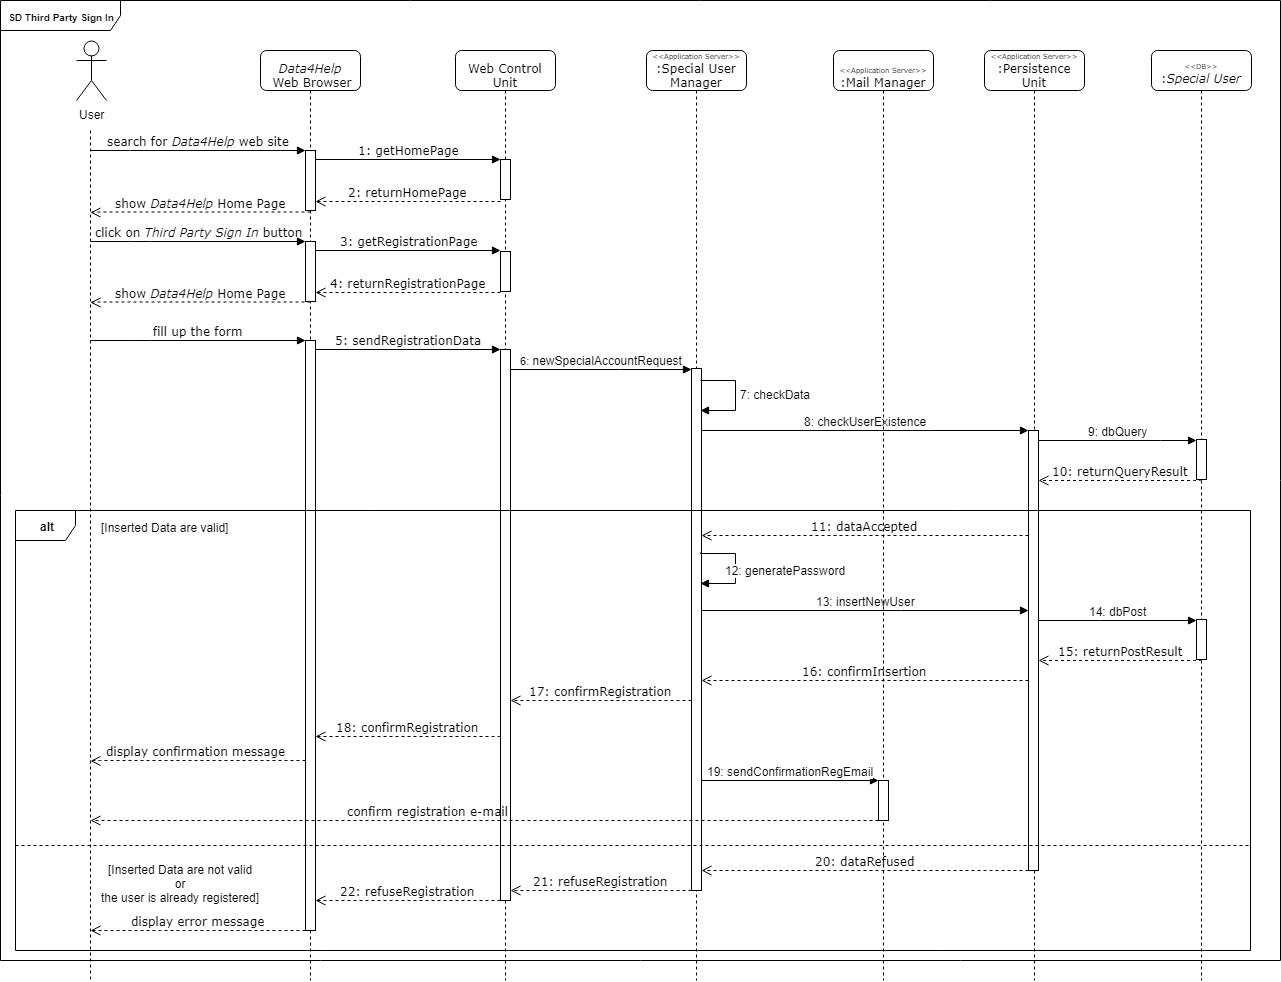
\includegraphics[width=\textwidth]{./img/sequence/webSignIn.png}
    \hspace{0.05\linewidth}
    \centering
    \caption{\textit{Third Party Sign In} sequence diagram: it is described the process through which a third party can register itself to \textit{Data4Help} services, obviously using \textit{Data4Help}'s web site, since it is the only available platform for third parties.}
		\label{img:webSignIn}
    \end{center}
\end{figure}

\begin{figure}[H]
  \begin{center}
  	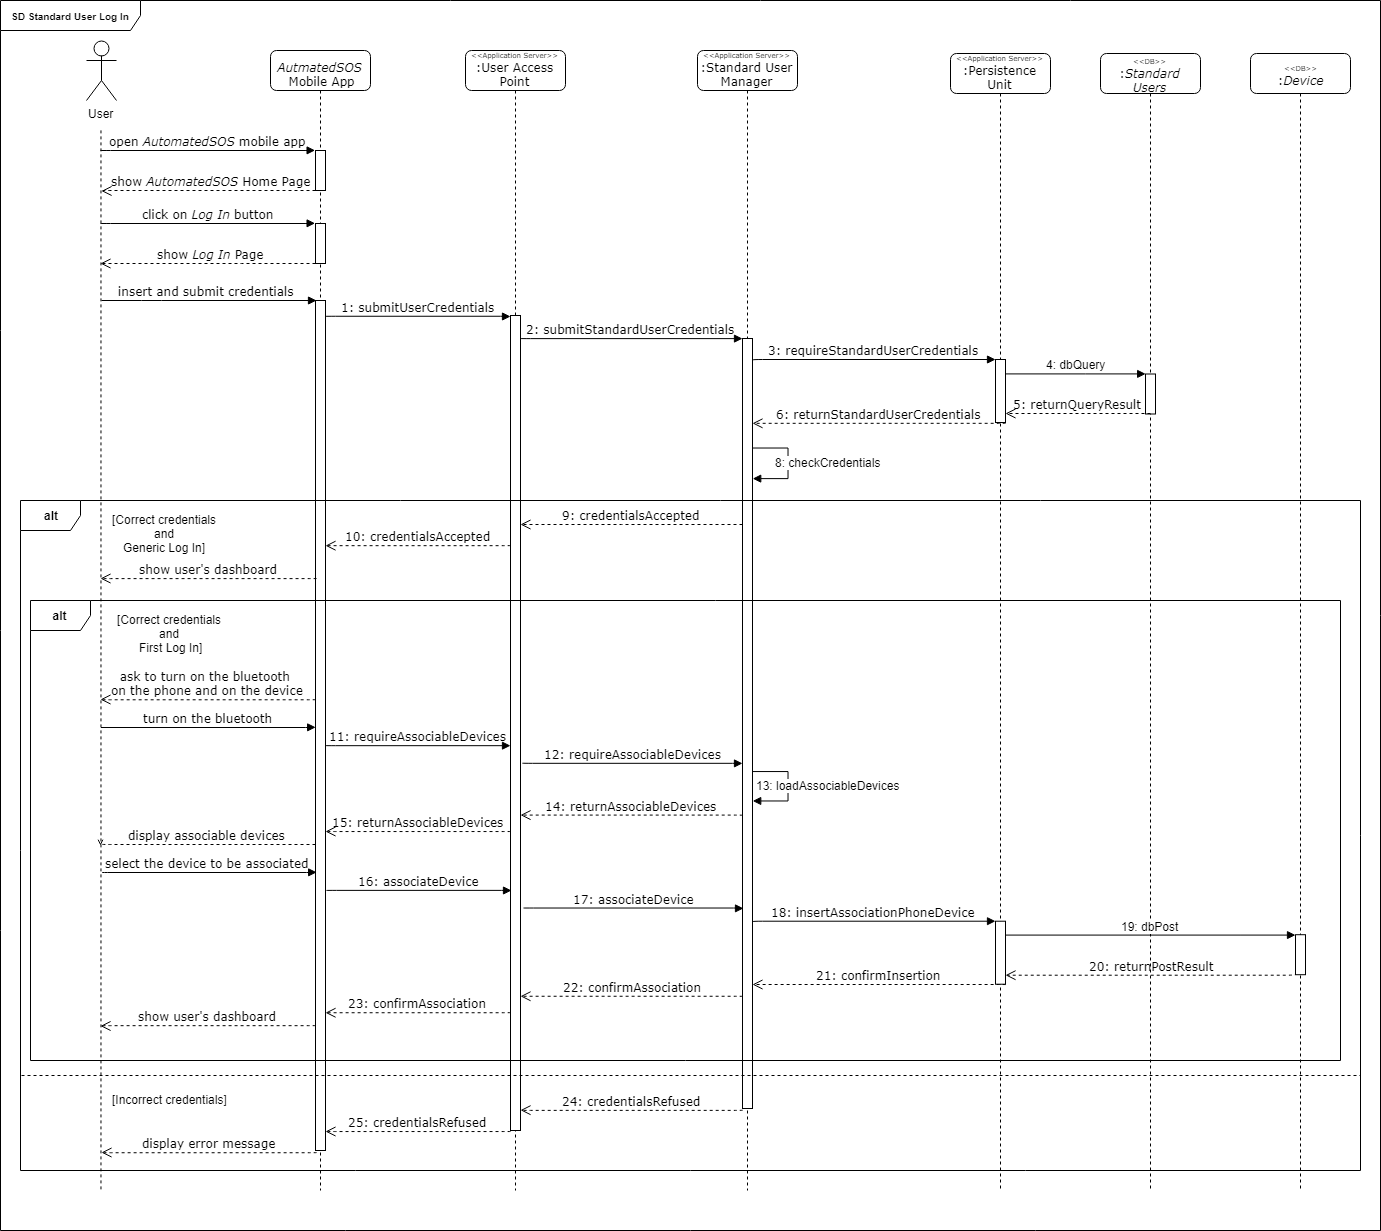
\includegraphics[width=\textwidth]{./img/sequence/appLogIn.png}
    \hspace{0.05\linewidth}
    \centering
    \caption{\textit{Standard User Log In} sequence diagram: it is described the process through which a standard user can access to \textit{AutomatedSOS} or \textit{Track4Run} applications.}
		\label{img:appLogIn}
    \end{center}
\end{figure}

\begin{figure}[H]
  \begin{center}
  	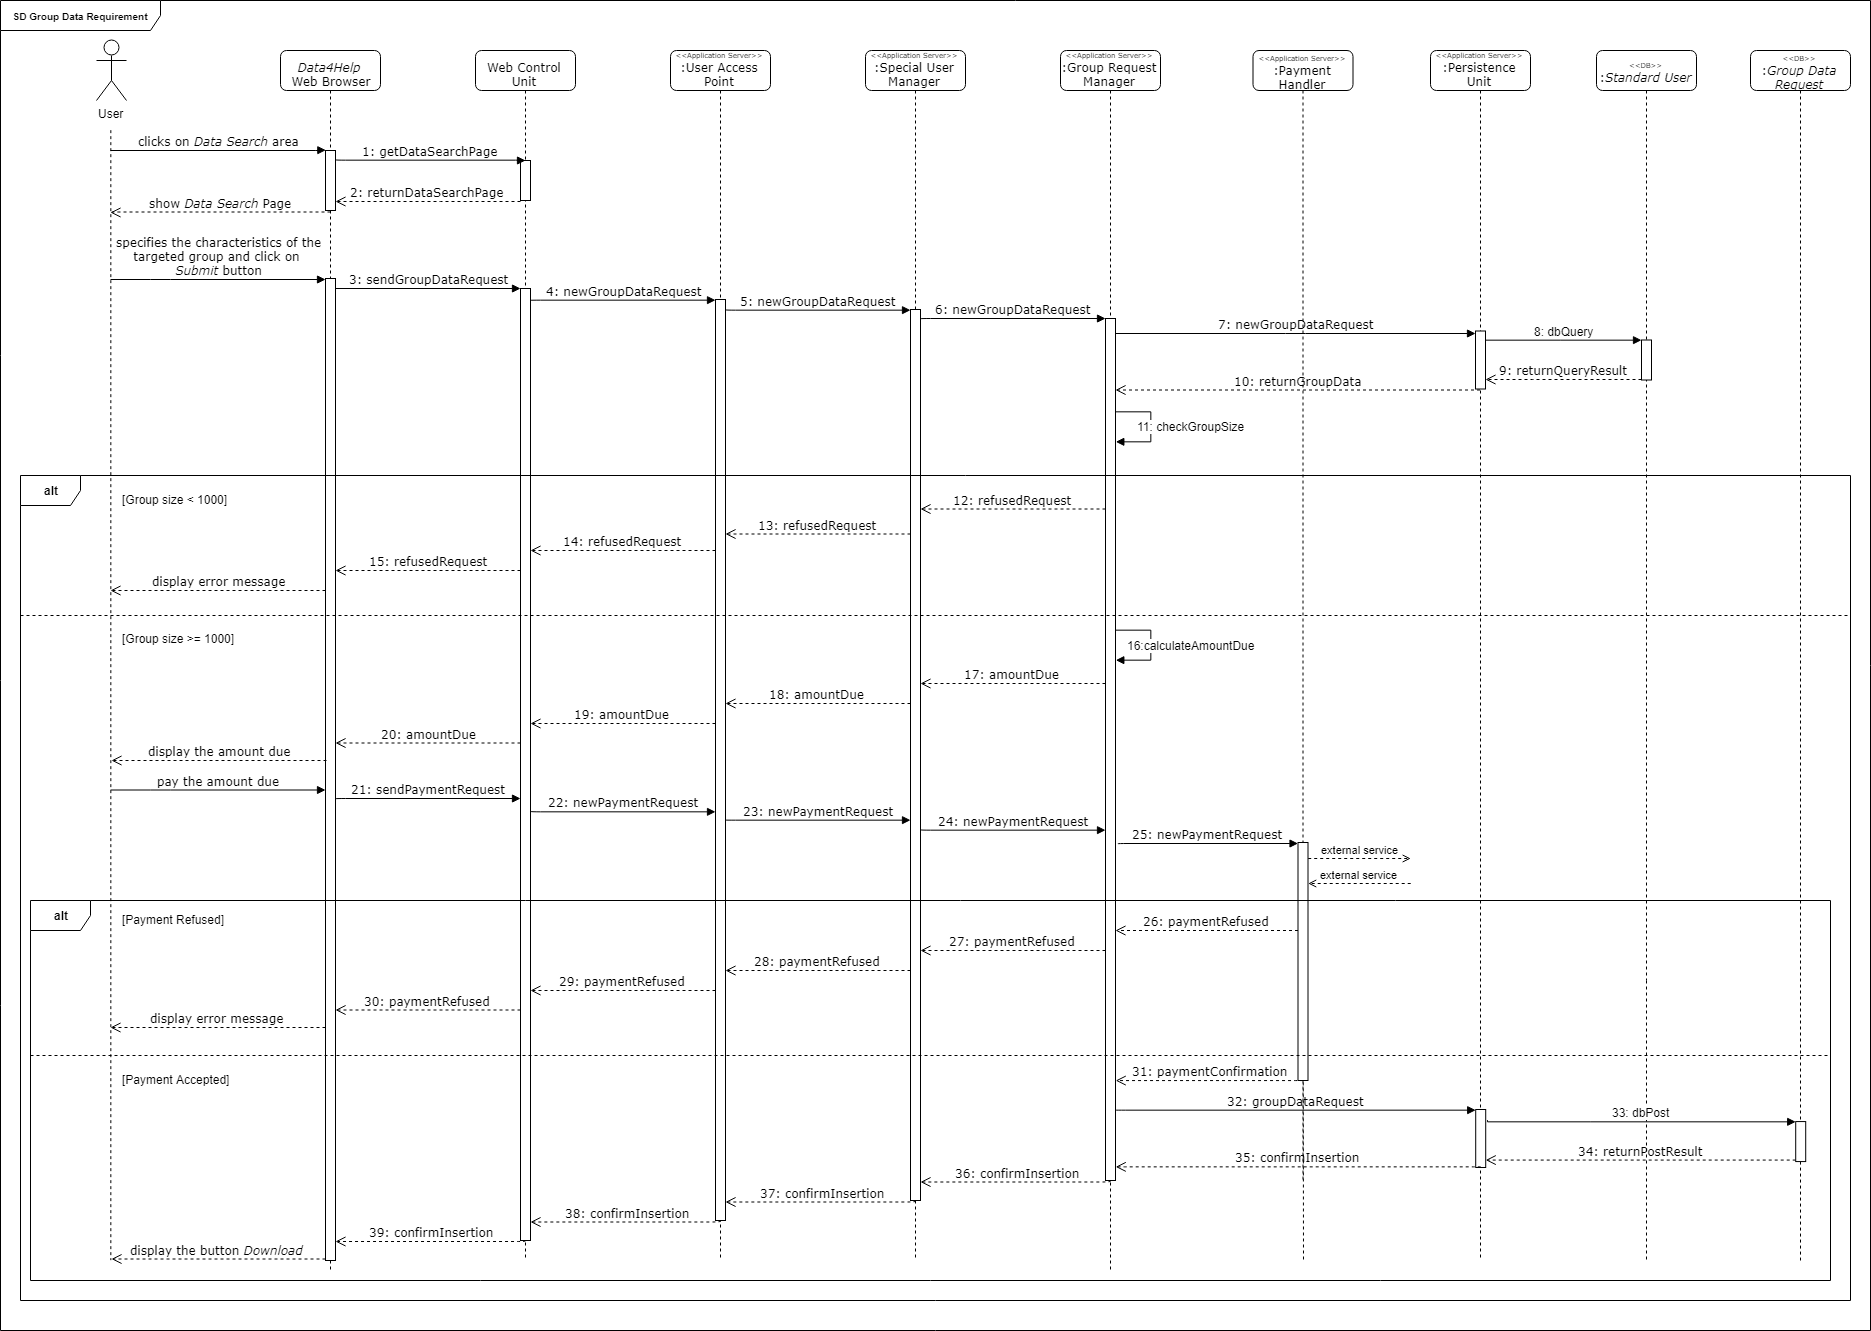
\includegraphics[width=\textwidth]{./img/sequence/groupDataRequest.png}
    \hspace{0.05\linewidth}
    \centering
    \caption{\textit{Group Data Request} sequence diagram: it is described the process through which a third party can require data of a group of people and then pay them.}
		\label{img:groupDataRequest}
    \end{center}
\end{figure}

\begin{figure}[H]
  \begin{center}
  	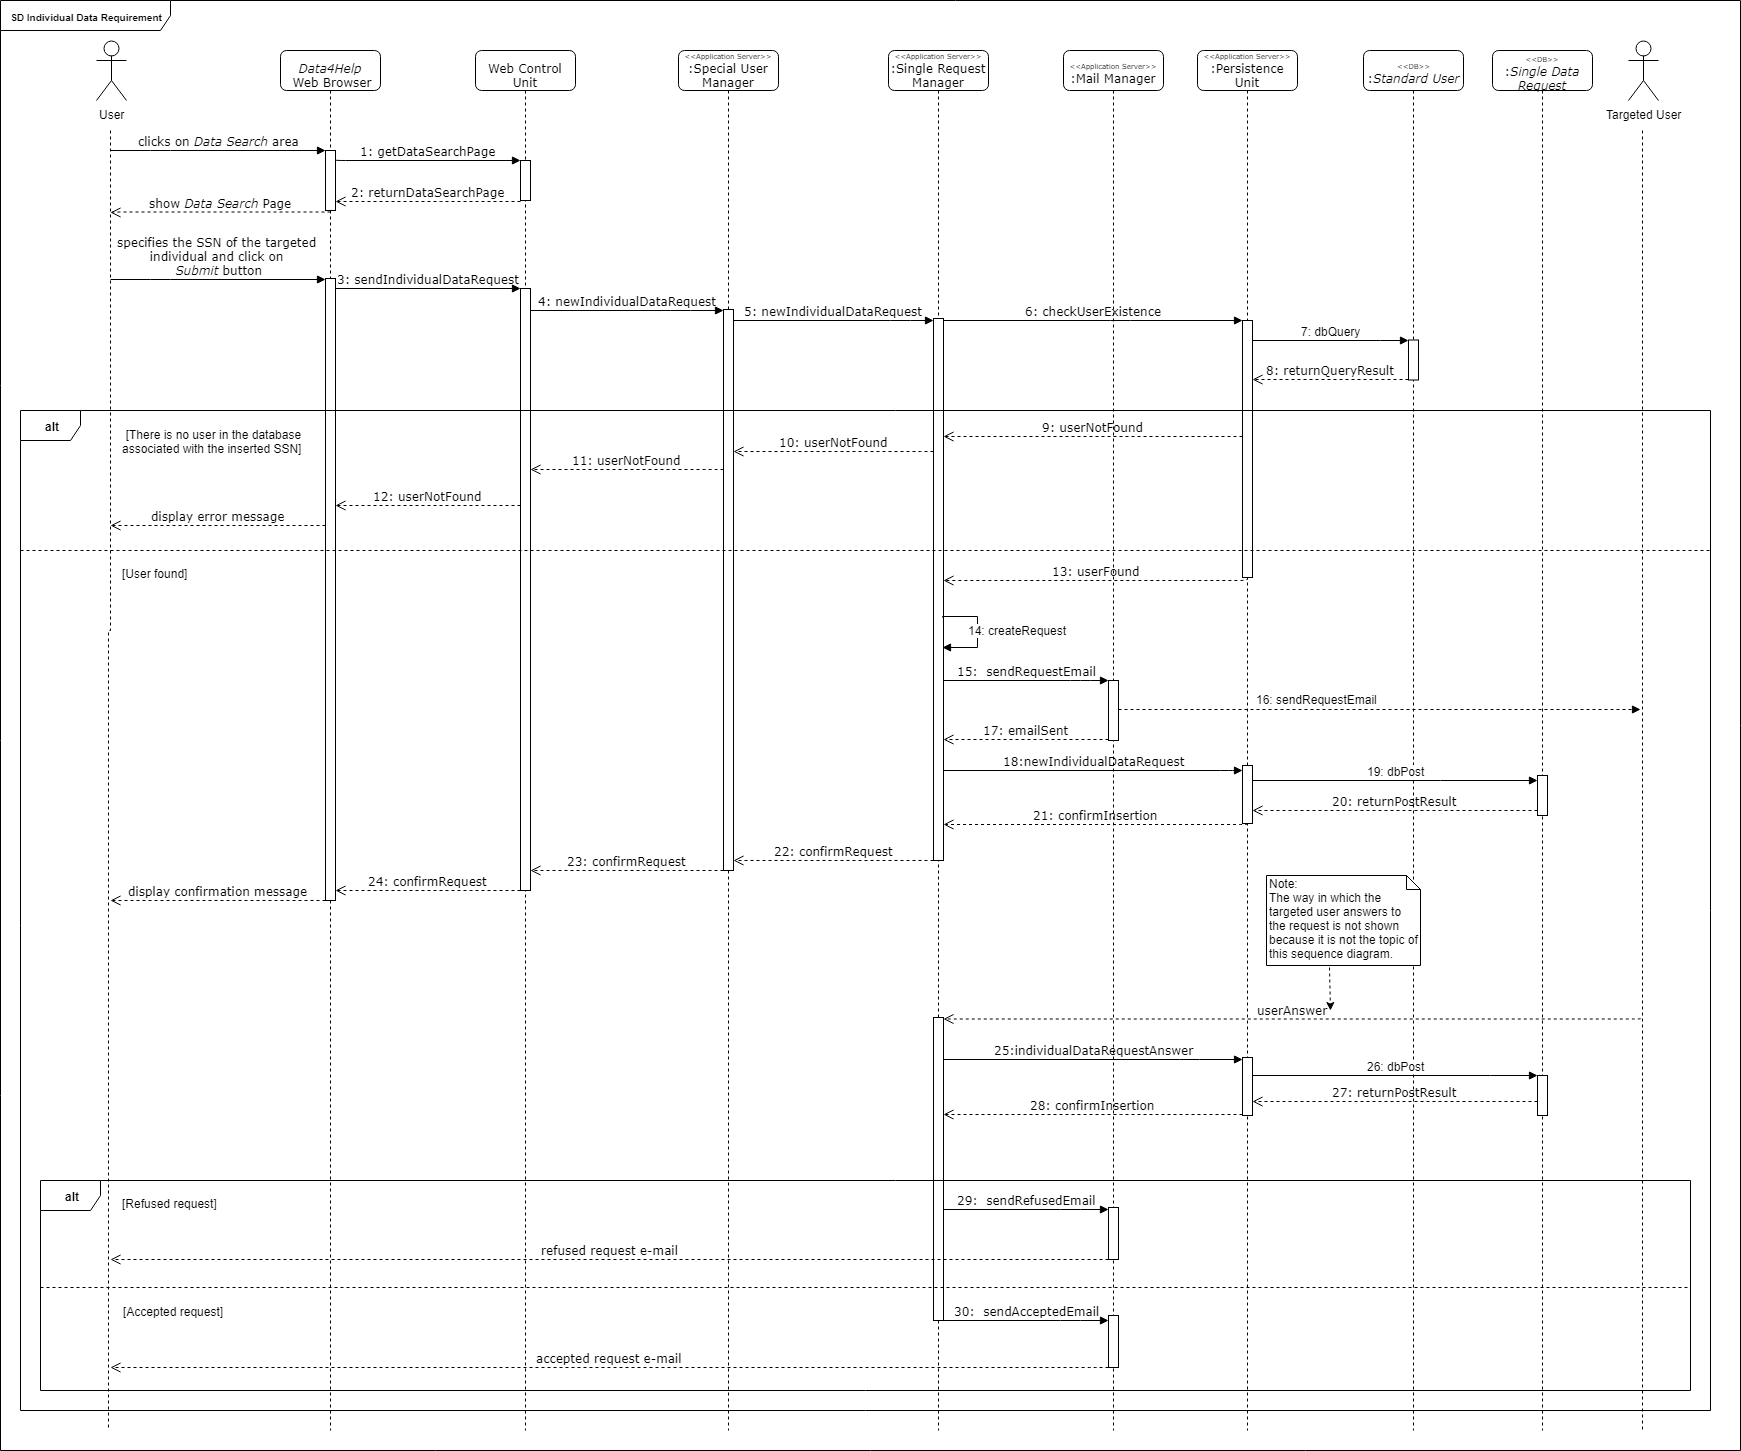
\includegraphics[width=\textwidth]{./img/sequence/individualDataRequest.png}
    \hspace{0.05\linewidth}
    \centering
    \caption{\textit{Individual Data Request} sequence diagram: it is described the process through which a third party can require data of an individual user and wait for a response. It is not described the way in which the targeted user answers to the request because it is not the topic of this sequence diagram. It is not even described the way in which the third party pays and eventually downloads the data because it is not considerable and it has just been explained in the \textit{Group Data Requst} sequence diagram.}
		\label{img:individualDataRequest}
    \end{center}
\end{figure}

\begin{figure}[H]
  \begin{center}
  	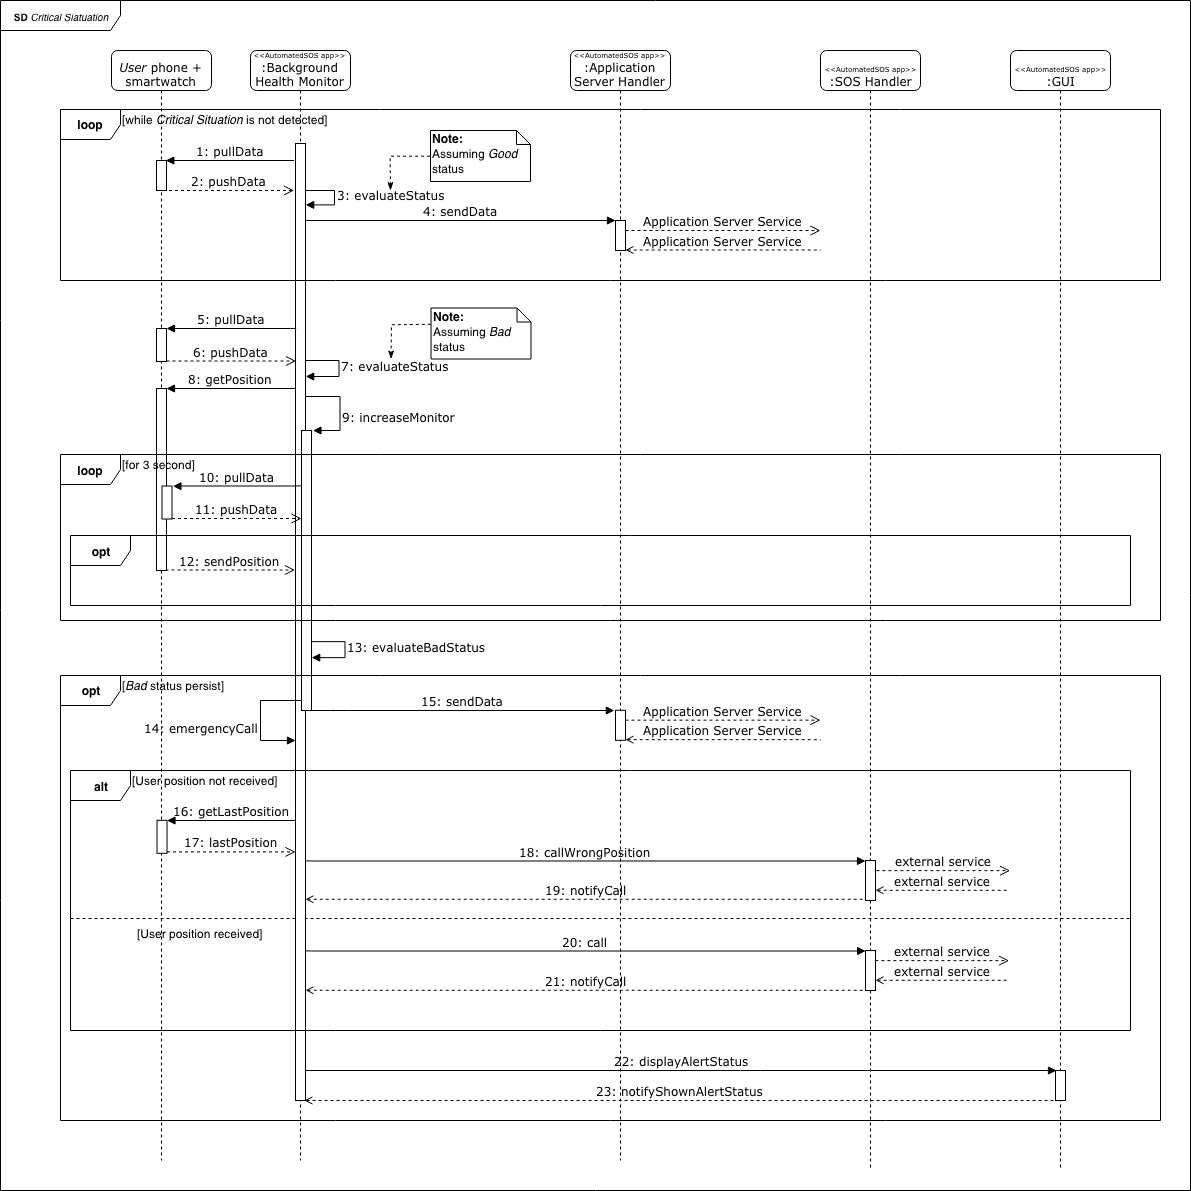
\includegraphics[width=\textwidth]{./img/sequence/criticalSituation.png}
    \hspace{0.05\linewidth}
    \centering
    \caption{\textit{Critical Situation} sequence diagram: it is described the process through which a critical situation is detected by \textit{AutomatedSOS} application + device. It is not described the way in which \textit{AutomatedSOS} application stored the acquired data because it is not considerable for this topic.}
		\label{img:criticalSituation}
    \end{center}
\end{figure}

\begin{figure}[H]
  \begin{center}
  	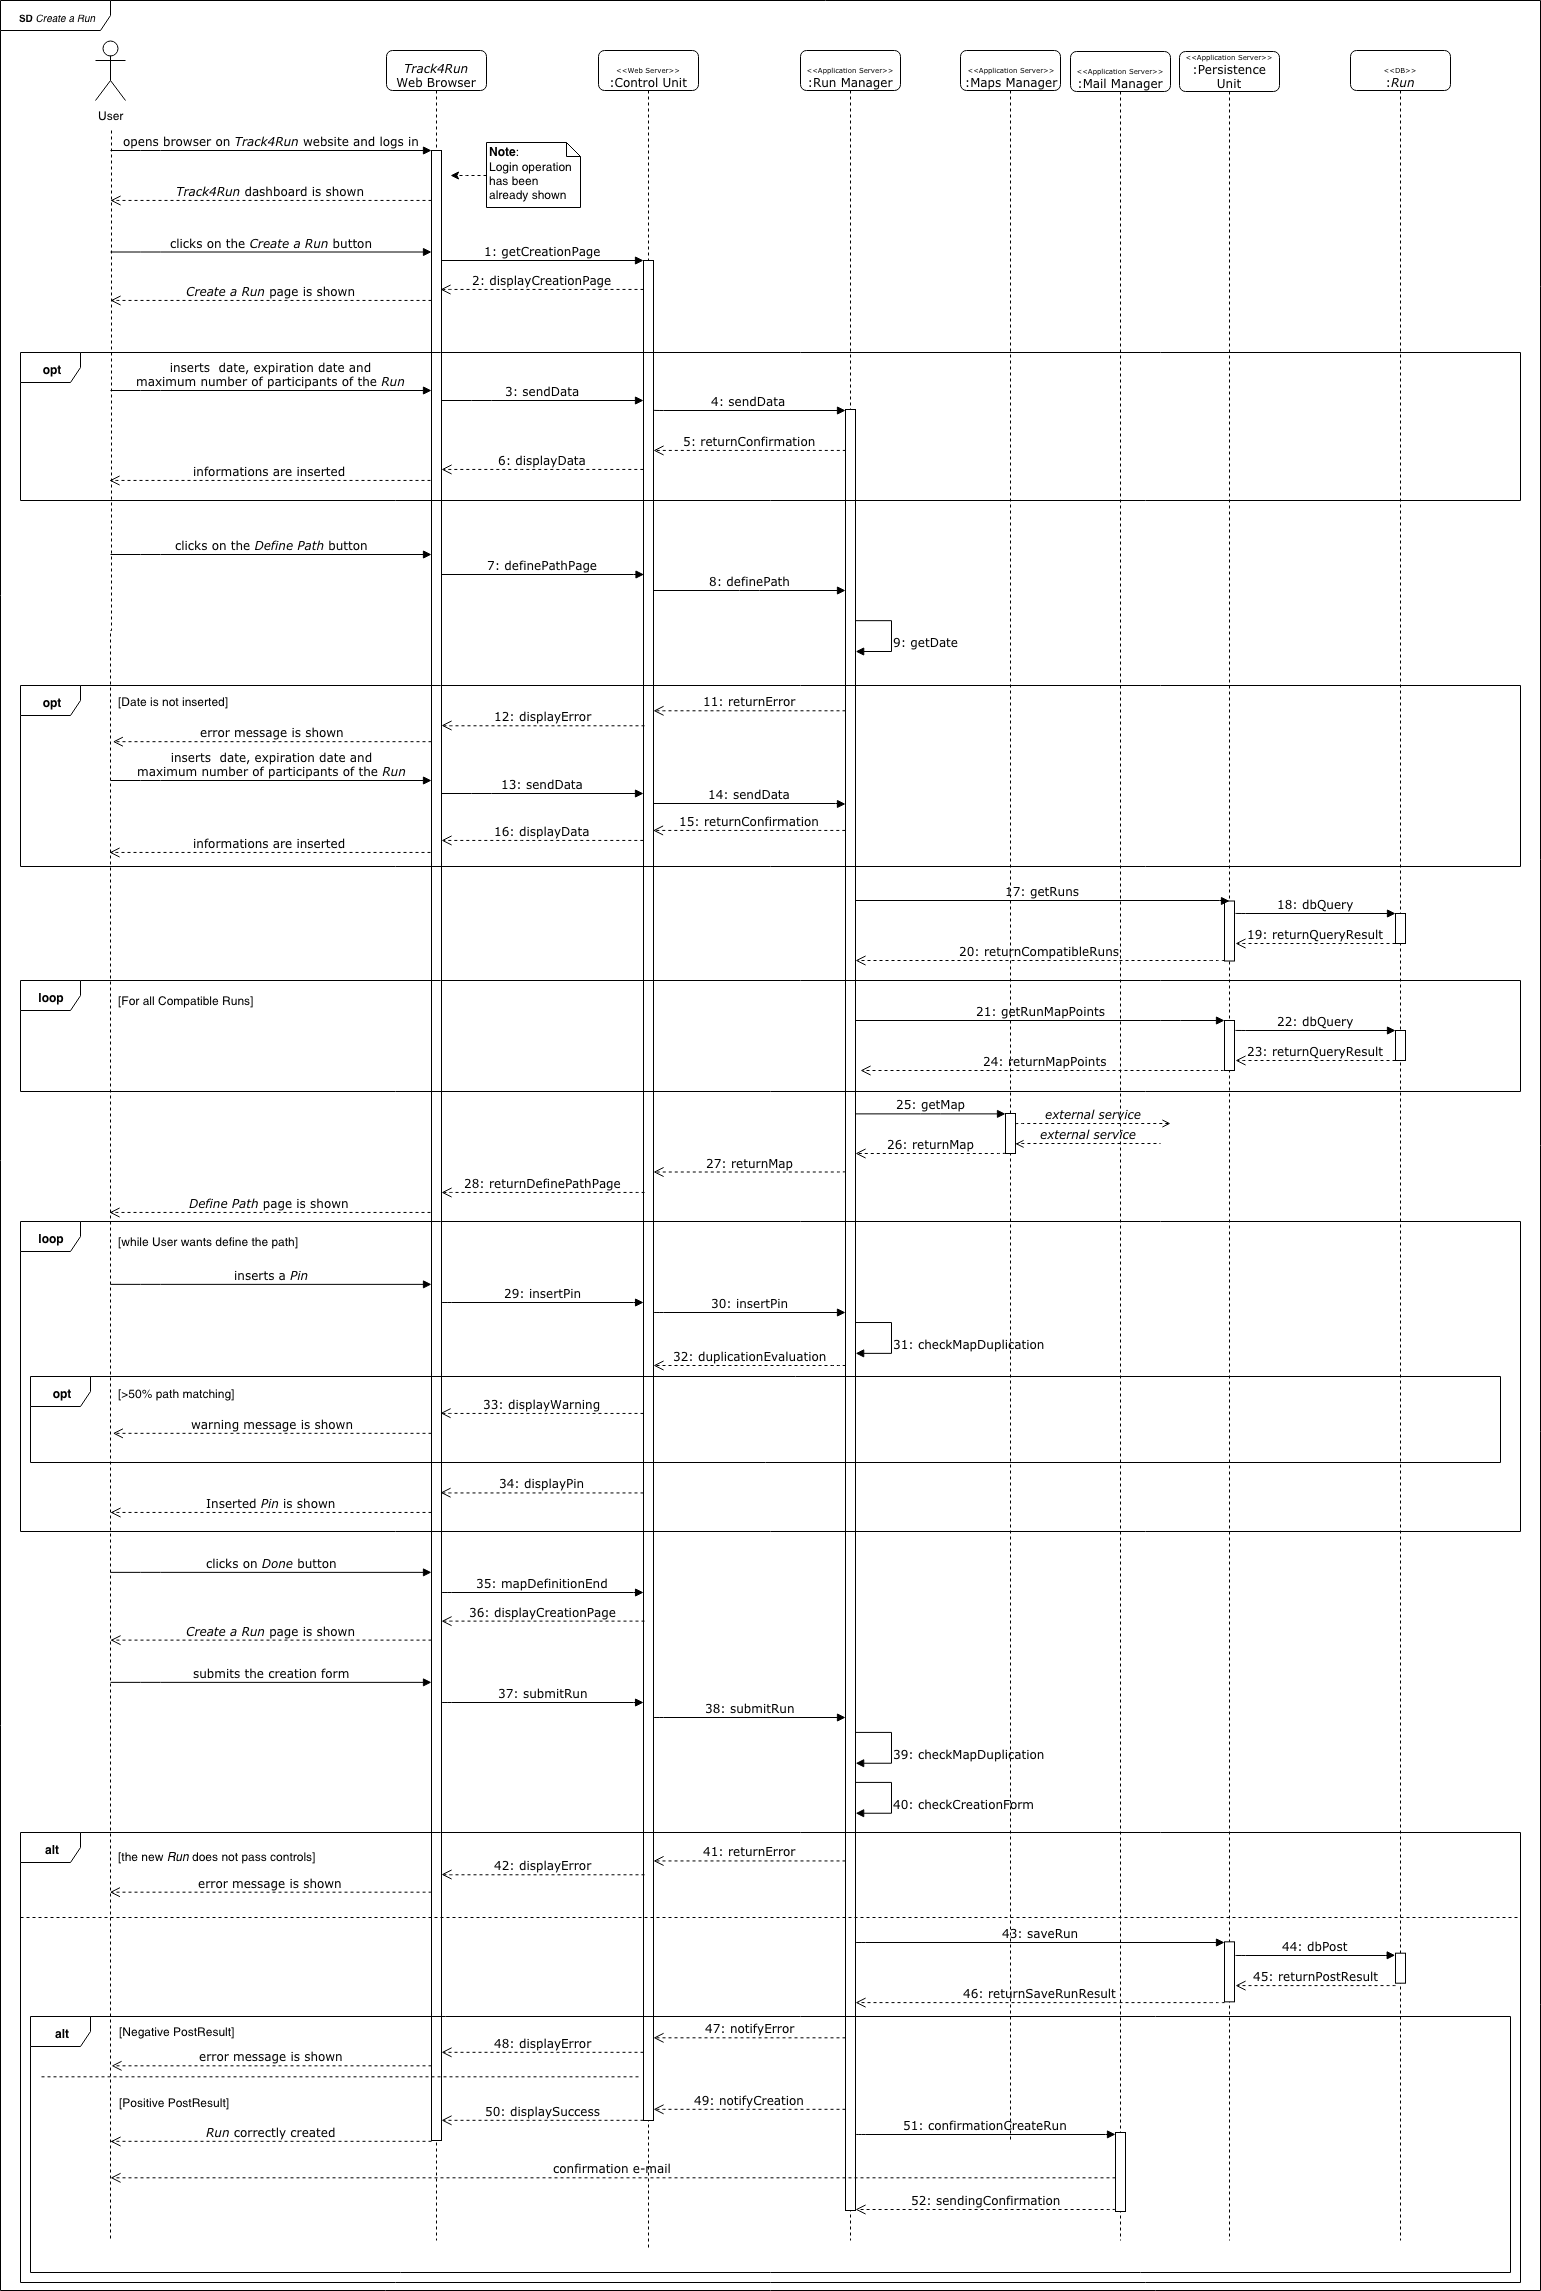
\includegraphics[height=.6\paperheight]{./img/sequence/createRun.png}
    \hspace{0.05\linewidth}
    \centering
    \caption{\textit{Create a Run} sequence diagram: it is described the process through which a standard user can create a new run.}
		\label{img:createRun}
    \end{center}
\end{figure}

\begin{figure}[H]
  \begin{center}
  	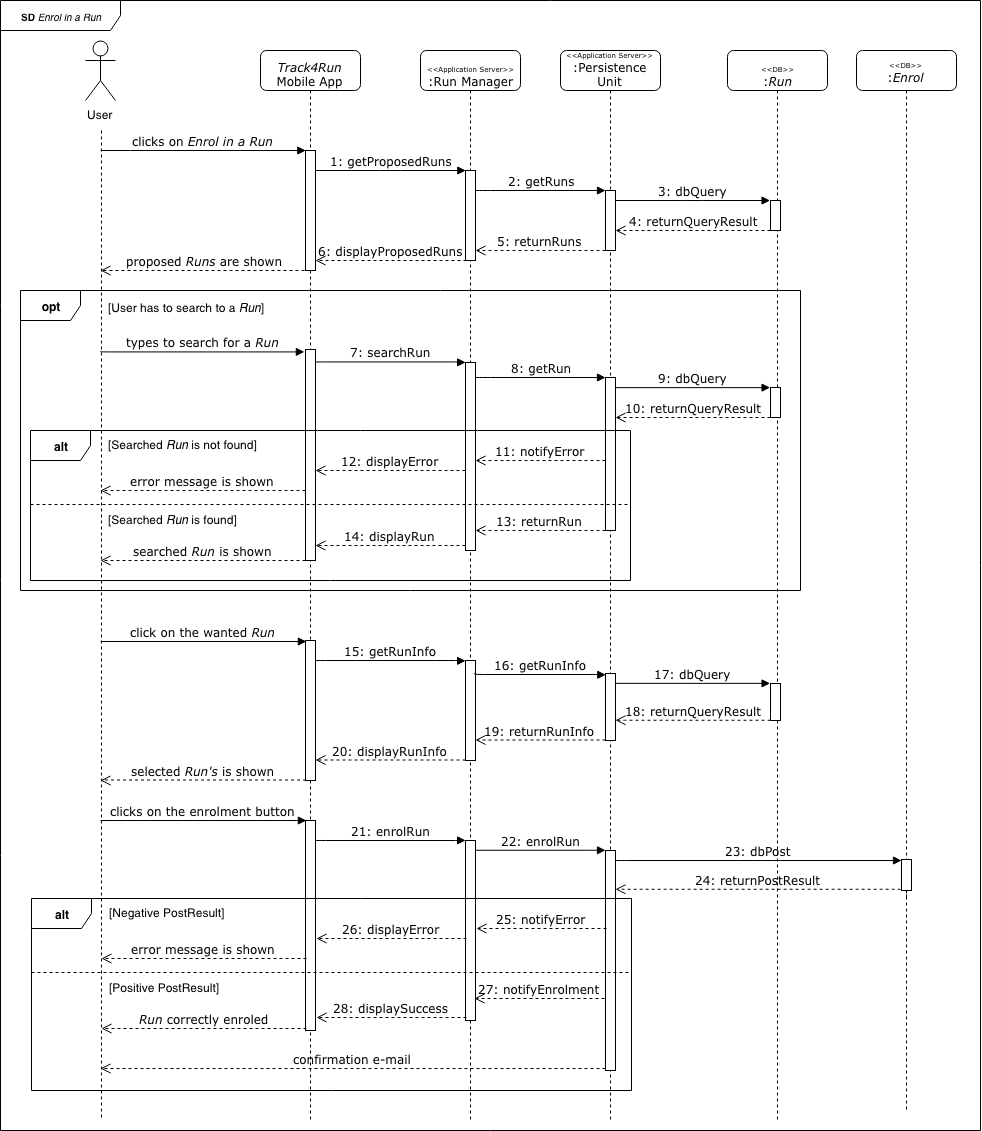
\includegraphics[width=\textwidth]{./img/sequence/enrolRun.png}
    \hspace{0.05\linewidth}
    \centering
    \caption{\textit{Enrol in a Run} sequence diagram: it is described the process through which a standard user can enrol himself/herself in a run. }
		\label{img:enrolRun}
    \end{center}
\end{figure}

\begin{figure}[H]
  \begin{center}
  	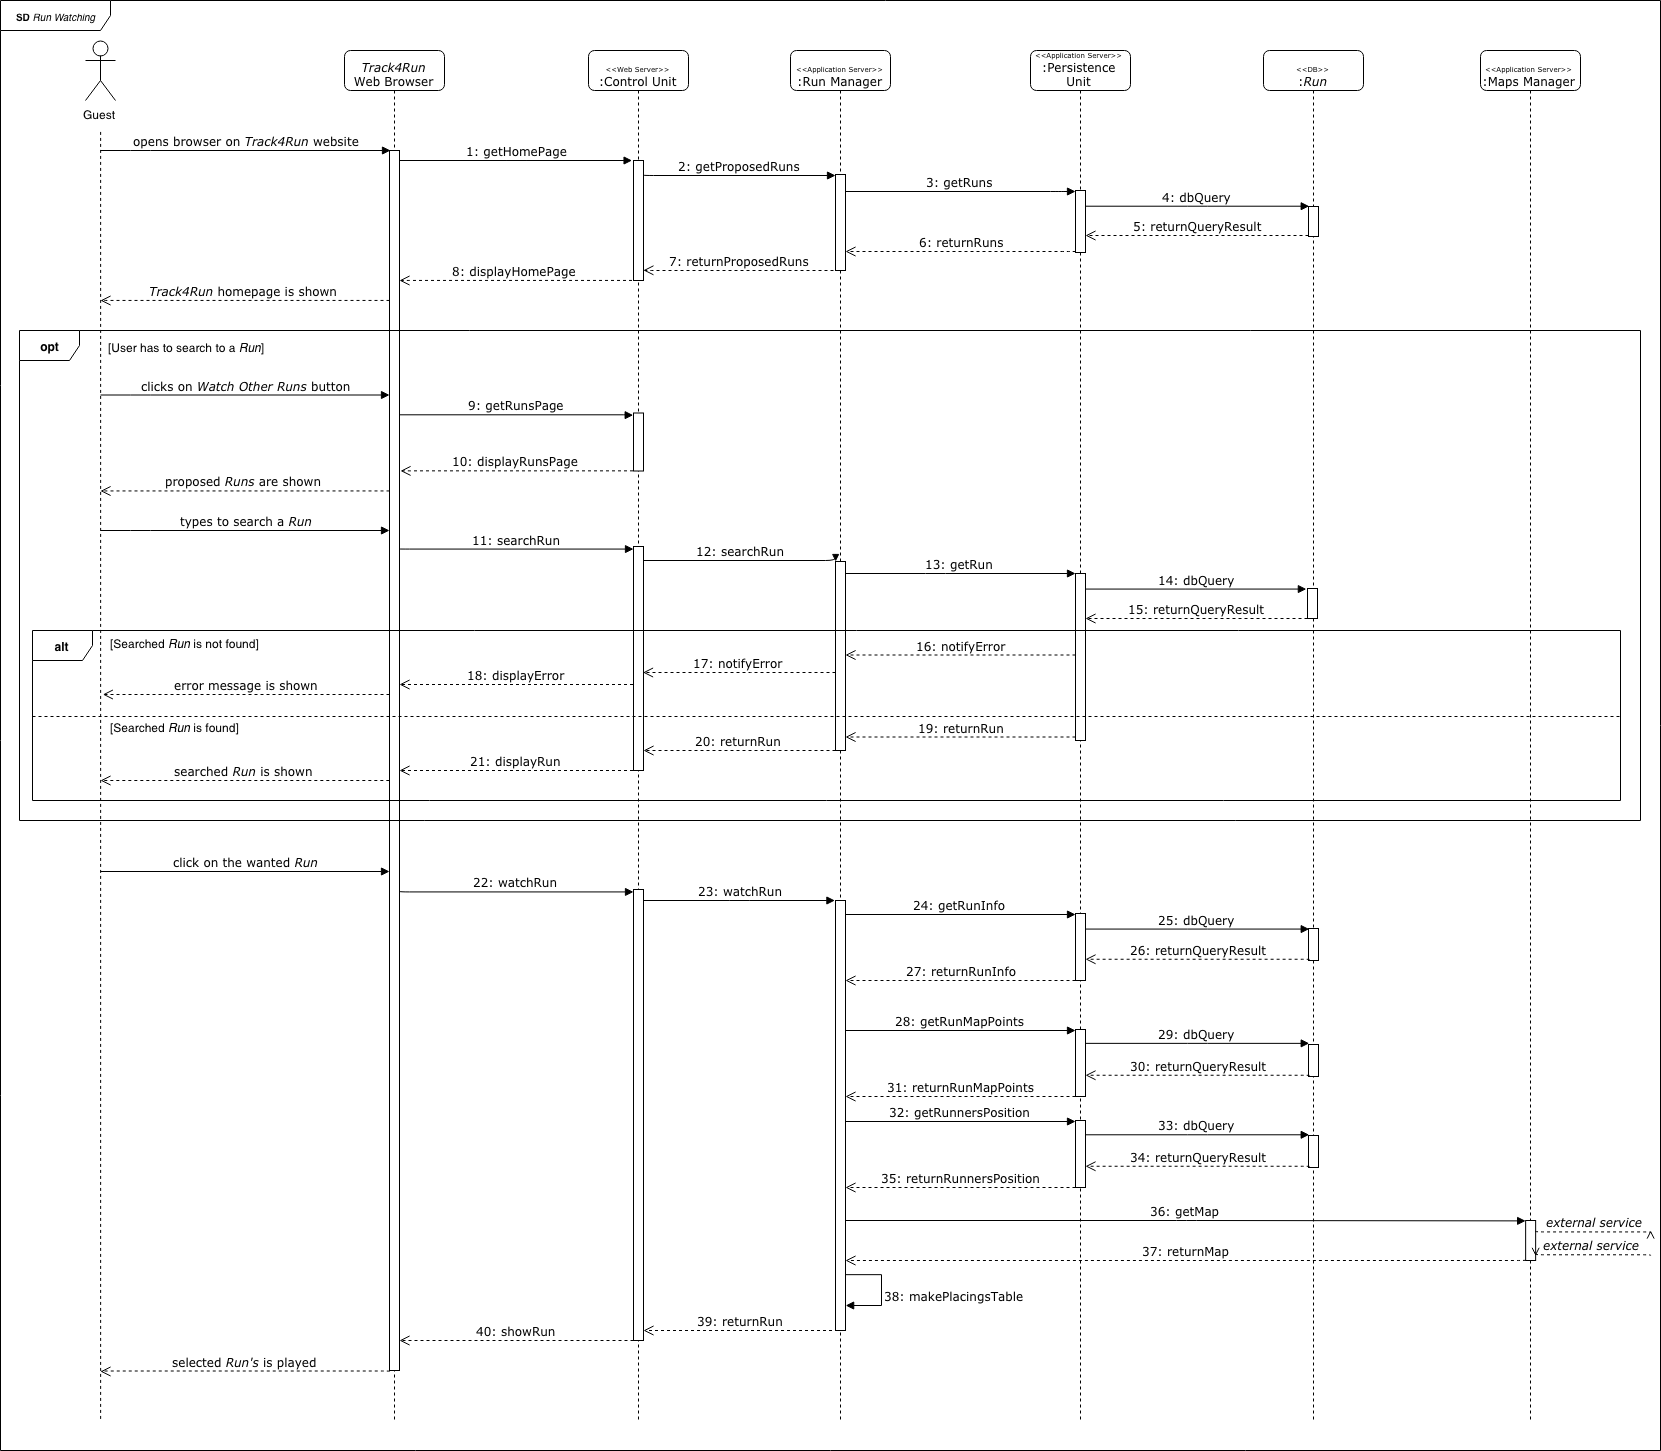
\includegraphics[width=\textwidth]{./img/sequence/watchRun.png}
    \hspace{0.05\linewidth}
    \centering
    \caption{\textit{Run Watching} sequence diagram: it is described the process through which a not registered user can watch a run. Notice that he/she can access directly to part of the \textit{Run Manager} services without any log in.}
		\label{img:watchRun}
    \end{center}
\end{figure}


\clearpage

\section{Component Interfaces}
This section contains some detailed informations about interfaces between components of the system.\\
A detailed description focuses the attention over the actions of a procedure of a certain component called by other components.\\
Huge part of these actions could be seen played in the \textit{Sequence Diagrams} (Section \ref{runtimeViewSection}).

\subsection{Application Server}

\subsubsection{Standard User Manager}
Following procedures are called by other components:
\begin{itemize}
  \item \textbf{associateDevice}\quad This procedure is used to associate a selected device with the smartphone in use.
  \item \textbf{changeDevice}\quad This procedure is called to start the process of changing the associated device.
  \item \textbf{changePassowrd}\quad This procedure is called to change the password of the user's account.
  \item \textbf{deleteProfile}\quad This procedure is called to delete the user's profile.
  \item \textbf{modifyPersonalInformations}\quad This procedure is called to modify personal informations (among the modifiable ones:  city of residence, address and occupation.)
  \item \textbf{newStandardAccountRequest}\quad This procedure is called to start a standard user registration process that can be then accepted or refused.
  \item \textbf{requireAssociableDevices}\quad This procedure is used to induce the system to load the list of associable devices.
  \item \textbf{submitStandardUserCredentials}\quad This procedure is called to let (or not) a standard user log in into one of \textit{Track Me} services.
\end{itemize}

\myparagraph{}
Following procedures are called internally to the component:
\begin{itemize}
  \item \textbf{checkCredentials}\quad This procedure is called to check whether the credentials inserted by the user during the login match with the ones saved in the system's database.
  \item \textbf{checkData}\quad This procedure is called to check if the user has inserted correctly all the required data.
  \item \textbf{generatePassword}\quad This procedure is called to generate a random password to be assigned to the newly created standard user.
  \item \textbf{loadAssociableDevices}\quad This procedure is called to load the list of associable devices.
\end{itemize}

\subsubsection{Special User Manager}
Following procedures are called by other components:
\begin{itemize}
  \item \textbf{changePassowrd}\quad This procedure is called to change the password of the special user's account.
  \item \textbf{deleteProfile}\quad This procedure is called to delete the user's profile.
  \item \textbf{modifyPersonalInformations}\quad This procedure is called to modify personal informations (among the modifiable ones:  legal address, billing address, corporate e-mail address, sector and all the data regarding the legal representative)
  \item \textbf{newGroupDataRequest}\quad This procedure is called to start the process of requiring data of a group of people and to send the useful data to the specialized component (\textit{Group Request Manager}).
  \item \textbf{newIndividualDataRequest}\quad This procedure is called to start the process of requiring to an individual user the sharing of his/her data and to send the useful data to the specialized component (\textit{Single Request Manager}).
  \item \textbf{newPaymentRequest}\quad This procedure is called to start the process of paying some required data calling the corresponding procedure on the more specialized component (\textit{Group Request Manager}).
  \item \textbf{newSpecialAccountRequest}\quad This procedure is called to start a special user registration process that can be then accepted or refused.
  \item \textbf{submitSpecialUserCredentials}\quad This procedure is called to let (or not) a special user log in into one of \textit{Track Me} services.
\end{itemize}

\myparagraph{}
Following procedures are called internally to the component:
\begin{itemize}
  \item \textbf{checkCredentials}\quad This procedure is called to check whether the credentials inserted by the special user during the login match with the ones saved in the system's database.
  \item \textbf{checkData}\quad This procedure is called to check if the special user has inserted correctly all the required data.
  \item \textbf{generatePassword}\quad This procedure is called to generate a random password to be assigned to the newly created special user.
\end{itemize}

\subsubsection{Group Request Manager}
Following procedures are called by other components:
\begin{itemize}
  \item \textbf{newGroupDataRequest}\quad This procedure is called to start the process of requiring data of a group of pepole.
  \item \textbf{newPaymentRequest}\quad This procedure is called to start the process of paying some required data calling the corresponding procedure on the dedicated component (\textit{Payment Handler}).
\end{itemize}

\myparagraph{}
Following procedures are called internally to the component:
\begin{itemize}
  \item \textbf{calculateAmountDue}\quad This procedure is called to calculate the amount due to download some required available data.
  \item \textbf{checkGroupSize}\quad This procedure is called to check whether the size of the required group of people is over 10000 or not.
\end{itemize}

\subsubsection{Single Request Manager}
Following procedures are called by other components:
\begin{itemize}
  \item \textbf{newIndividualDataRequest}\quad This procedure is called to start the process of requiring to an individual user the sharing of his/her data.
  \item \textbf{newPaymentRequest}\quad This procedure is called to start the process of paying some required data calling the corresponding procedure on the dedicated component (\textit{Payment Handler}).
\end{itemize}

\myparagraph{}
Following procedures are called internally to the component:
\begin{itemize}
  \item \textbf{calculateAmountDue}\quad This procedure is called to calculate the amount due to download some required available data.
  \item \textbf{createRequest}\quad This procedure is called to generate a sharing data request that has to be sent to an individual user.
\end{itemize}

\subsubsection{Mail Manager}
Following procedure is called by other components:
\begin{itemize}
  \item \textbf{confirmationEmail}\quad This procedure sends a confirmation e-mail to the user.
  \item \textbf{sendAcceptedEmail}\quad This procedure is called to inform a third party that an individual user, of which it has required the data, has accepted its request and so data will be immediatly available after completing the payment.
  \item \textbf{sendRefusedEmail}\quad This procedure is called to inform a third party that an individual user, of which it has required the data , has refused its request.
  \item \textbf{sendRequestEmail}\quad This procedure is called to send a sharing data request to an individual user.
\end{itemize}

\subsubsection{Maps Manager}
Following procedure is called by other components:
\begin{itemize}
  \item \textbf{getMap}\quad This procedure retrives a map from the external service.
\end{itemize}

\subsubsection{Run Manger}
Following procedures are called by other components:
\begin{itemize}
  \item \textbf{checkCreationForm}\quad This procedure checks all the fields of a creation for \textit{Create a Run} form.
  \item \textbf{definePath} \quad This procedure is called to open the path definition interface and to prepare the system to manage avoiding of maps duplications.
  \item \textbf{deleteEnrolement} \quad This procedure allow a user to delete an enrolment in a \textit{Run}.
  \item \textbf{deleteRun} \quad This procedure allow a user to delete a \textit{Run}.
  \item \textbf{enrolRun} \quad This procedure allow a user to enrol in a \textit{Run}.
  \item \textbf{getProposedRuns} \quad This procedure is called to retrive \textit{Runs} to propose to the users.
  \item \textbf{getRunInfo} \quad This procedure is called to retrive information of a particular \textit{Run}.
  \item \textbf{insertPin} \quad This procedure is called to insert a \textit{Pin} on a map during hte definition of a path.
  \item \textbf{makePlacingsTable} \quad This procedure is called to create the \textit{Placings Table} of a given \textit{Run} knowing path and runners' position.
  \item \textbf{searchRun} \quad This produce is called to search a given \textit{Run}.
  \item \textbf{sendData} \quad This procedure is used to submit data informations of a \textit{Run} and these data are used to compute functional requirement expecially for the \textit{Create a Run} use case (for instance avoiding 50\% of map duplication).
  \item \textbf{submitRun} \quad This produce is called when a \textit{User} has defined a \textit{Run} and wants to publish it.
  \item \textbf{watchRun} \quad This procedure is called to watch a given \textit{Run}.
\end{itemize}

\myparagraph{}
Following procedures are called internally to the component.
\begin{itemize}
  \item \textbf{checkMapDuplication} \quad This procedure is called to check the duplication of a given path with the compatible ones.
  \item \textbf{getDate} \quad This procedure is used to get the inserted \textit{Date} during the \textit{Create a Run} phase.
\end{itemize}

\subsubsection{Persistence Unit}
Following procedures are called by other components:
\begin{itemize}
  \item \textbf{checkExistingUser}\quad This procedure queries the credentials of a specific user to check whether they are already present in the database or not.
  \item \textbf{deleteEnrolement} \quad This procedure deletes an enrolment of a user on the DB through the DBMS.
  \item \textbf{deleteRun} \quad This procedure deletes a \textit{Run} on the DB through the DBMS.
  \item \textbf{enrolRun}\quad This procedure posts an enrolment of a user on the DB through the DBMS.
  \item \textbf{getRun}\quad This procedure queries required \textit{Run} on the DB through the DBMS.
  \item \textbf{getRunInfo}\quad This procedure queries required \textit{Run}'s information on the DB through the DBMS.
  \item \textbf{getRunMapPoints}\quad This procedure queries required \textit{Run path} on the DB through the DBMS.
  \item \textbf{getRunnersPosition}\quad This procedure queries \textit{Runners} position of a certain \textit{Run} on the DB through the DBMS.
  \item \textbf{getRuns}\quad This procedure queries required \textit{Runs} on the DB through the DBMS.
  \item \textbf{groupData}\quad This procedure queries the data of a specified group of people on the DB through the DBMS.
  \item \textbf{individualDataRequestAnswer}\quad This procedure posts the answer recieved by an individual user for an individual data request on the DB through the DBMS.
  \item \textbf{insertAssociationPhoneDevice}\quad This procedure posts a new association phone-device on the DB through the DBMS.
  \item \textbf{insertNewUser}\quad This procedure posts a new user on the DB through the DBMS.
  \item \textbf{newGroupDataRequest}\quad This procedure posts a new group data request on the DB through the DBMS.
  \item \textbf{newIndividualDataRequest}\quad This procedure posts a new individual data request on the DB through the DBMS.
  \item \textbf{requireSpecialUserCredentials}\quad This procedure queries the credentials of a special user (its email-password) to check if they correspond with the ones inserted during the login.
  \item \textbf{requireStandardUserCredentials}\quad This procedure queries the credentials of a standard user (his/her email-password) to check if they correspond with the ones inserted during the login.
  \item \textbf{saveRun}\quad This procedure posts a new \textit{Run} on the DB through the DBMS.
\end{itemize}

\subsubsection{Payment Handler}
Following procedures is called by other components:
\begin{itemize}
  \item \textbf{newPaymentRequest}\quad This procedure is called to pay some required data, it calls the dedicated external service.
\end{itemize}

\subsection{AutomatedSOS}
\subsubsection{Application Server Handler}
Following procedures are called by other components:
\begin{itemize}
  \item \textbf{getData}\quad This procedure is called to get data information of the user from the DB via \textit{Application Server}.
  \item \textbf{login}\quad This procedure is called to log in \textit{AutomatedSOS}.
  \item \textbf{sendData}\quad This procedure is called to send data information of the user to the \textit{Application Server} and store them into the DB.
\end{itemize}

\subsubsection{Background Health Monitor}
Following procedures are called by other components:
\begin{itemize}
  \item \textbf{lastPosition}\quad This procedure is called to send the last \textit{User}'s position to \textit{AutomatedSOS}.
  \item \textbf{pushData}\quad This procedure is called to send data that \textit{AutomatedSOS} has to evaluate.
  \item \textbf{sendPosition}\quad This procedure is called to send user's position to \textit{AutomatedSOS}.
\end{itemize}

\myparagraph{}
Following procedures are called internally to the component.
\begin{itemize}
  \item \textbf{evaluateBadStatus}\quad This procedure is called when the system is in an \textit{Alerted Status} and has to evaluate if it has to call an ambulance or the \textit{Alerted Status} was generated from an abnormal measure.
  \item \textbf{evaluateStatus}\quad This procedure evaluates the data received from the user's device.

  \item \textbf{increaseMonitor}\quad This procedure is called at the \textit{Alerted Status} beginning to increase the life paramethers detection.
\end{itemize}

\subsubsection{Health Status Manager}
Following procedures are called by other components:
\begin{itemize}
  \item \textbf{makeStatistics}\quad This procedure is called to get data informations of the user and makes weekly and monthly statistics to visualize.
\end{itemize}

\subsubsection{GUI}
Following procedures are called by other components:
\begin{itemize}
  \item \textbf{displayAlertStatus}\quad This procedure shows on the smartphone's screen the emergency call in progress.
  \item \textbf{displayDashboard}\quad This procedure shows on the smartphone's screen the dashboard of a logged user.
  \item \textbf{displayLogin}\quad This procedure shows on the smartphone's screen the login page.
  \item \textbf{displayStatistics}\quad This procedure shows on the smartphone's screen the statistics' page of a logged user.
\end{itemize}

\myparagraph{}
Following procedures are called internally to the component.
\begin{itemize}
  \item \textbf{logout}\quad This procedure logs out the user and gets back to the \textit{Login} page of the application.
\end{itemize}

\subsubsection{SOS Handler}
Following procedures are called by other components:
\begin{itemize}
  \item \textbf{call}\quad This produce call an ambulance and send it the user's position.
  \item \textbf{callWrongPosition}\quad This produce call an ambulance notifying that there is an error in getting the user's position and the lastone is sended.
\end{itemize}


\section{Selected Architectural Styles and Patterns}\label{architecturalStyle}
Following are the choices made regarding architectural styles and patterns.

\subsection{Client and Server}
A client server architecture was chosen for system implementation.
This allows the exchange of information between Internet-connected devices used by users and the centralized server that collects data and offers Data4Help services.
In particular:
\begin{itemize}
  \item The AutomatedSOS and Track4Run applications installed on users' devices are clients connected to the application server that receives and processes data.
  \item The desktop web browsers used by users (both standard and special) to access the services offered by Data4Help are clients that communicate with the Web Server that provides an HTTPS interface.
  \item The application server is seen as a server by the web browser and as a client by the application server that allows it to process requests.
  \item The application server is seen as a server from the web server and applications installed on smartphones and as a client from the database that receives and processes its requests (queries).
  \item The database is seen as a server by the application server that sends the requests and waits for the answers.
\end{itemize}

\subsection{Multi-tiered architecture}
A multi-tiered client-server architecture is used to ensure the separation between the MVC model levels (model, view, controller).
In this way a greater stability of the system is also guaranteed:
\begin{itemize}
  \item In case of failure of the application server, the applications installed on users' devices continue to work and collect data. However, AutomatedSOS is able to make an emergency call. This also applies if the device is temporarily without an Internet connection (but with emergency calls available). Once the application server or Internet connection has been restored, the device will reconnect and send the data collected during the period of absence of the service to the server.
  \item In case of failure of the web server, the application server remains active and the applications installed on users' devices continue to work correctly (and to send data correctly to the server). The services offered through the use of the web browser will not be available.
\end{itemize}

\subsection{Thin Client}
The services accessible through web browsers are considered thin clients because the software used does not install software belonging to Data4Help.
All the necessary information required to use the service is offered by the Web Server through HTTPS, including a graphical interface and application logic.
Also, the Track4Run app is considered thin client because the application that provides the graphical user interface is installed on the phone but most of the application logic (and in particular the one used to manage the races) is based on the application server to which it connects.

\subsection{Thick Client}
The Automated SOS app is to be considered as a thick client in fact in the app in addition to the graphical interface and the logic related to the acquisition of user data, there is also the logic that allows the phone to make a call to the external service used for handling emergency calls.
Thanks to this the app is able to detect a state of emergency and alert the ambulance even if the connection with the server is not available.

\subsection{Model-View-Control}
The MVC model allows to identify three main components in the management of a client-server application. They are the Model, the View and the Controller.
The following diagram shows the management of these three levels according to the use of thin or thick clients (\ref{img:client_server}).

\begin{figure}[H]
  \begin{center}
  	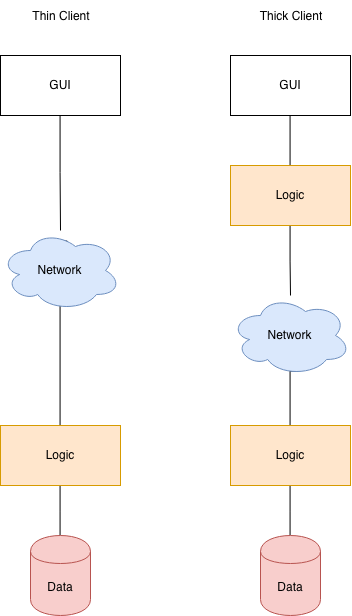
\includegraphics[width=0.4\textwidth]{./img/client_server.png}
    \hspace{0.05\linewidth}
    \centering
    \caption{Possible management of the client-server connection according to the MVC model. Thin or thick client.}
		\label{img:client_server}
    \end{center}
\end{figure}


\section{Other Design Decisions}
\subsection{User authentication}
In order to guarantee the confidentiality of user data, access to the system, both for standard users and for special users, takes place by entering a username and password.
The username used for access coincides with the email address used during registration.

\subsection{Password storing}
The passwords chosen by the users are saved in the database after being encrypted using a SHA512 algorithm.
In this way, the password to be used for accessing Data4Help services is not stored in plaintext in the user database, but it is a transformation from which, even with very powerful computers, it is very difficult to trace the original password.
In this way even using the normal Internet connection, if an intruder could pick up the string containing the password, he would not be able to trace the password used to access the service.

\subsection{Security in the transfer of information}
The transfer of data between the clients and the server is done using the most modern data encryption systems.
For example, the Web Server offers an HTTPS interface to the Web Browser.

\subsection{Maps}
In order to manage the rides offered by Track4Run, the external Google Maps service is used.
Longitude and latitude are used to locate a position within the map.
To ensure a better service to the user who is responsible for creating the race, it is also given the opportunity to create the route using the features provided by Google Maps such as search by address, search for places of public interest, and so on. In the database the race course will still be saved as a sequence of positions in terms of longitude and latitude.

\subsection{Emergency call}
Emergency calls are handled using an external service.
This ensures that even in the event that the data network is not available, or the application server is out of service, it is still possible to call for help.
In fact, the external service works via the Internet or, in the absence of a connection, via SMS.
When the Automated SOS application detects an anomaly, it invokes the external service and sends it the location of the device and a precompiled text containing information related to the health of the user.
This information is then sent to the rescue service by the external service.

\clearpage

%User Interface Design
\chapter{User Interface Design}
\section{UX Diagrams}
The purpose of this section is to show the possible screens that the user might encounter during the use of the system.
The displayed information and the possible interactions by the user are also shown in these diagrams.\\
To allow a better reading of the diagrams themselves, they have been divided into 4 parts:
\begin{itemize}
  \item Diagram of Data4Help (accessible from Web Wrowser), Figure \ref{img:Data4Help}.
  \item Diagram of Track4Run (accessible from Web Wrowser), Figure \ref{img:Track4RunWeb}.
  \item Diagram of Track4Run (accessible from the App on Smartphone), Figure \ref{img:Track4RunApp}.
  \item Diagram of AutomatedSOS (accessible from the App on Smartphone), Figure \ref{img:AutomatedSOSApp}.
\end{itemize}
The AutomatedSOS diagram contains a screen unreachable by the user. It is the screen that is displayed when an emergency is detected and then an ambulance is alerted. For this screen to be displayed, the user must be logged in to the app and have connected a device.

\begin{figure}[H]
  \begin{center}
  	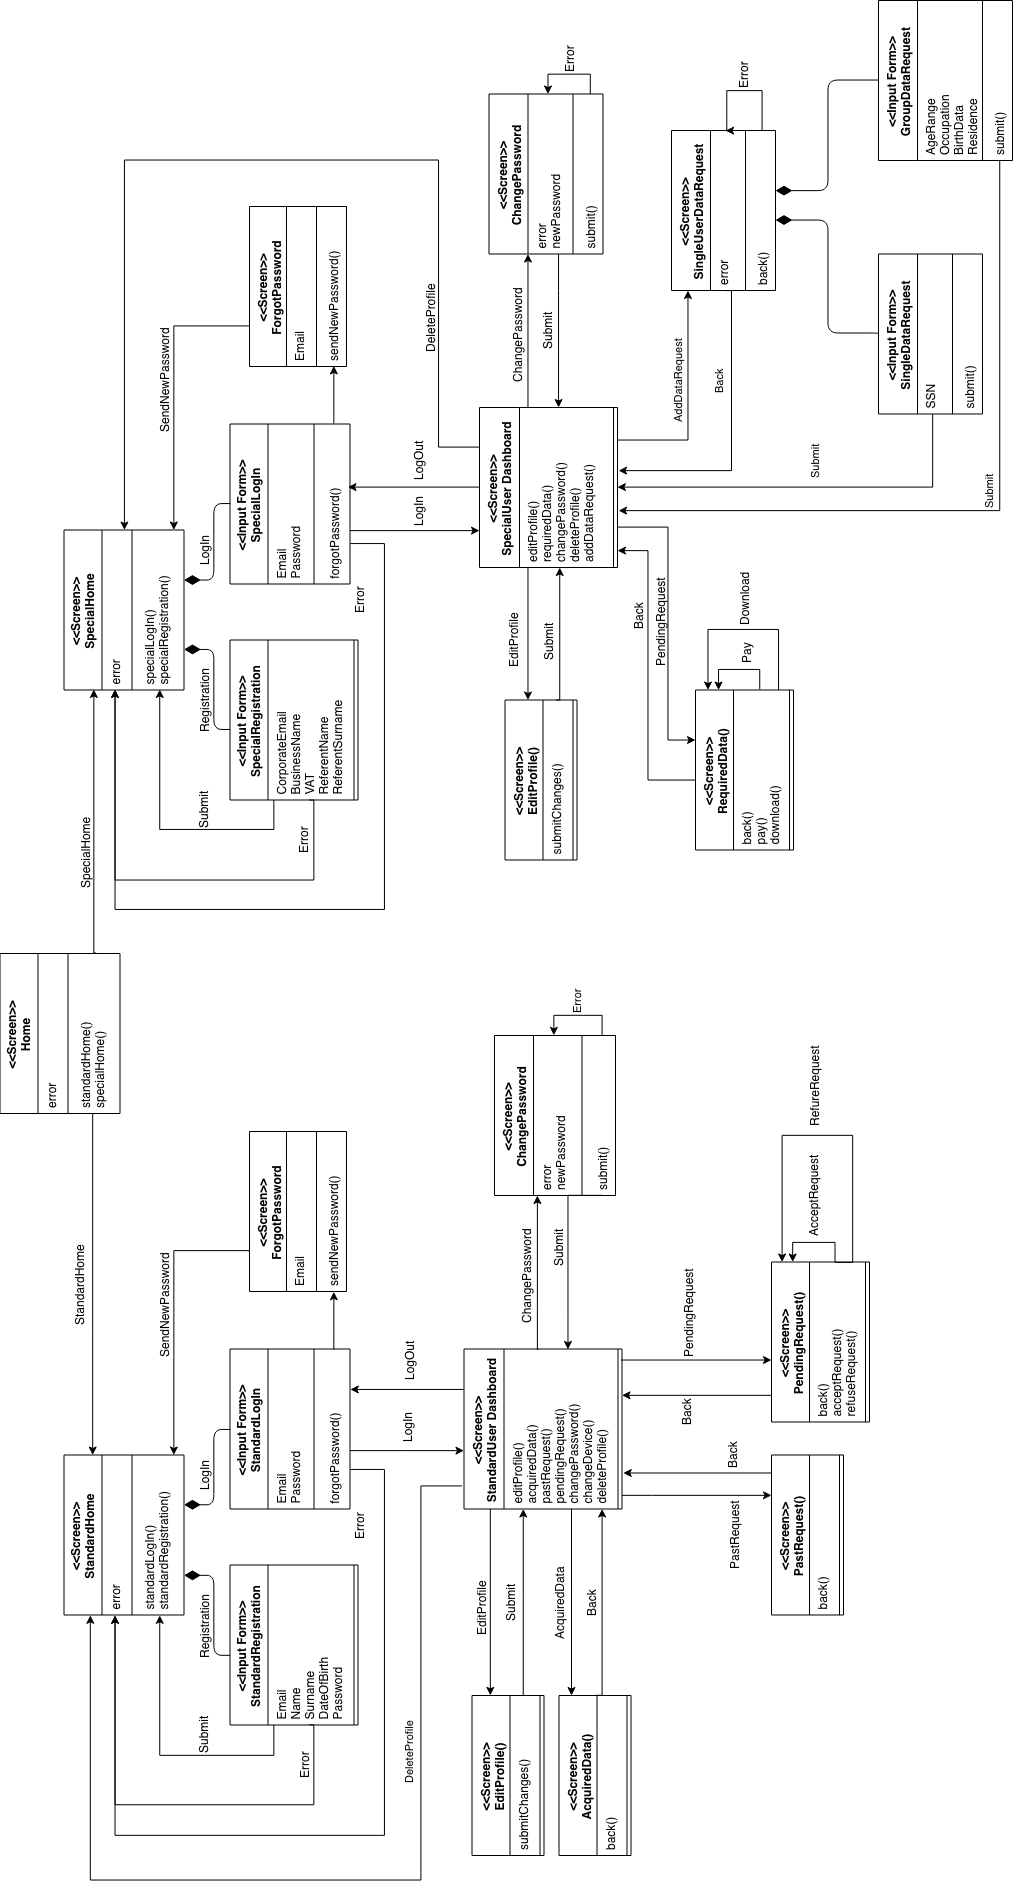
\includegraphics[height=0.68\paperheight]{./img/UXDiagram/UX_Diagram_Data4Help.png}
    \hspace{0.05\linewidth}
    \centering
    \caption{UX Diagram \textit{Data4Help} (Web)}
		\label{img:Data4Help}
    \end{center}
\end{figure}

\begin{figure}[H]
  \begin{center}
  	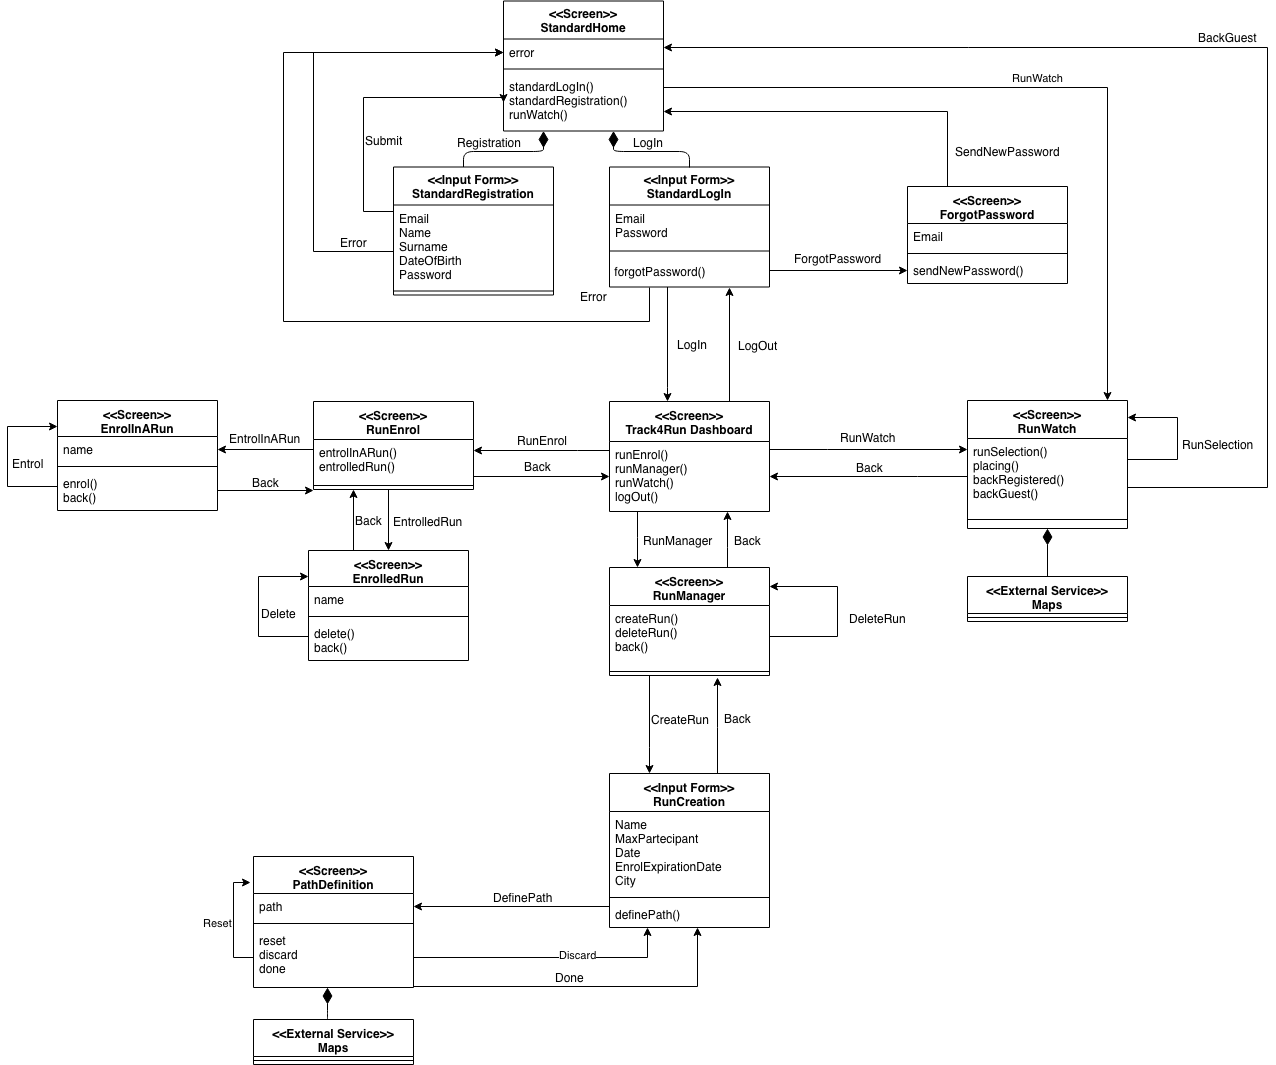
\includegraphics[width=0.68\paperwidth]{./img/UXDiagram/UX_Diagram_Track4Run_Web.png}
    \hspace{0.05\linewidth}
    \centering
    \caption{UX Diagram \textit{Track4Run} (Web)}
		\label{img:Track4RunWeb}
    \end{center}
\end{figure}

\begin{figure}[H]
  \begin{center}
  	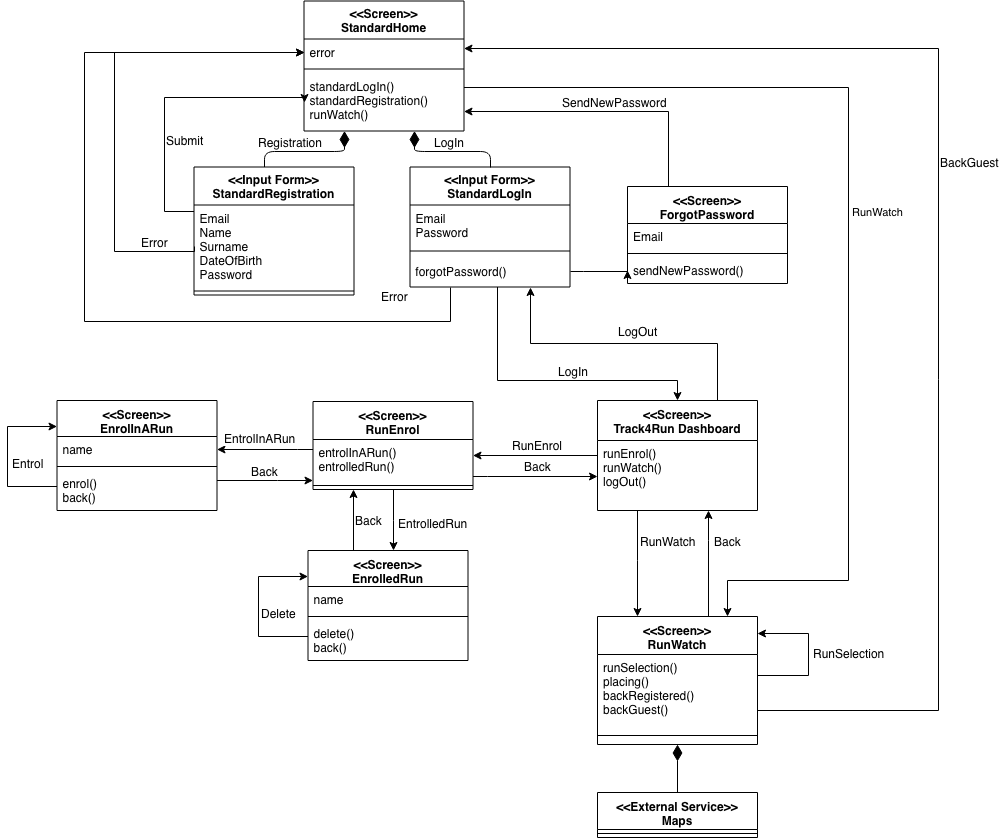
\includegraphics[width=0.68\paperwidth]{./img/UXDiagram/UX_Diagram_Track4Run_App.png}
    \hspace{0.05\linewidth}
    \centering
    \caption{UX Diagram \textit{Track4Run} (App)}
		\label{img:Track4RunApp}
    \end{center}
\end{figure}

\begin{figure}[H]
  \begin{center}
  	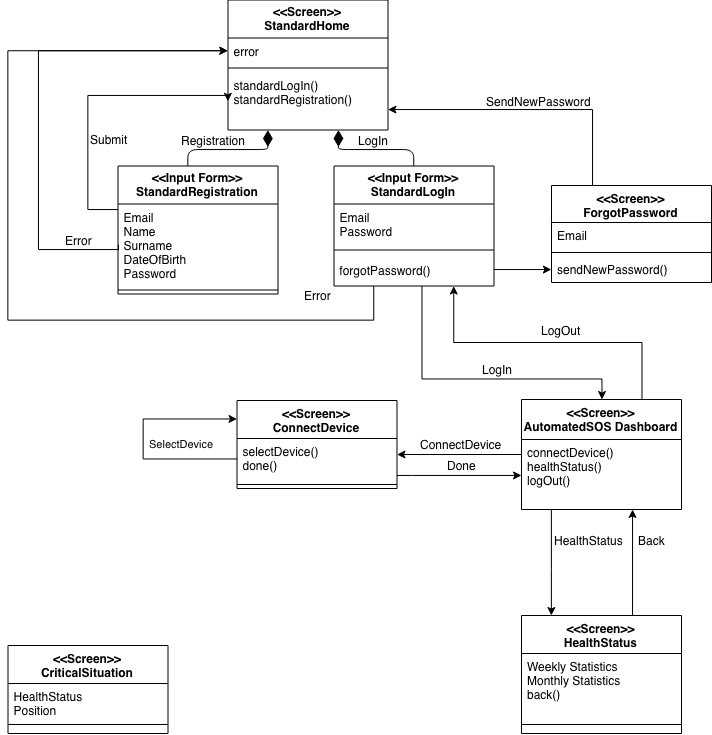
\includegraphics[width=0.68\paperwidth]{./img/UXDiagram/UX_Diagram_AutomatedSOS_App.png}
    \hspace{0.05\linewidth}
    \centering
    \caption{UX Diagram \textit{AutomatedSOS} (App)}
		\label{img:AutomatedSOSApp}
    \end{center}
\end{figure}

\section{User Interfaces}
For user interfaces, please refer to the Requirements Analysis and Specification Document where the mockups have been included and explained.

\clearpage

%Requirements Traceability
\chapter{Requirements Traceability}
\section{Functional Requirements}
In the table \ref{table:functionalRequirements} below it is highlighted the mapping between DD components and RASD goals and functional requirements. Notice that it is missing the component \textit{Persistence Unit} because the aim of the table is to focus on application logic components while the \textit{Persistence Unit} is only an interface with the database's DBMS.

\section{AutomatedSOS Functional Requirements}
Since there is a part of logic in the \textit{AutomatedSOS} application (explained in section \ref{architecturalStyle}) there is an additional table below (\ref{table:automatedFunctionalRequirements}), dedicated to \textit{AutomatedSOS} specific components with the correspondig achived goals and requirements.

\begin{center}
\begin{table}[H]
\begin{tabular}{|p{0.07\textwidth} | p{0.43\textwidth} | p{0.5\textwidth}|}
  \hline
    \textbf{Goal} & \textbf{DD Component} & \textbf{RASD Requirements} \\ \hline
     1 \newline 2 \newline 3 & Special User Manager & 3.2.2 Third Party Sign In \newline 3.2.4 Third Party Log In \newline 3.2.6 Manage Third Party Profile \\ \hline
     1 \newline 2 \newline 3 & Standard User Manager & 3.2.1 Individual Sign In \newline 3.2.3 Individual Log In \newline 3.2.5 Manage Profile \newline 3.2.7 Individual Data Requirement\\ \hline
     4 & Single Request Manager & 3.2.7 Individual Data Requirement\\ \hline
     5 & Group Request Manager & 3.2.8 Group Data Requirement\\ \hline
     6 & Data Collector Service Manager & 3.2.7 Individual Data Requirement \newline 3.2.8 Group Data Requirement \\ \hline
     9 \newline  10 \newline 11 \newline 12 \newline 13 \newline 14 \newline 15 & Run Manager & 3.2.11 Create a Run \newline 3.2.12 Delete a Run \newline 3.2.13 Enrol in a Run \newline 3.2.14 Delete an Enrolment in a Run \newline 3.2.15 Run Watching\\ \hline
     10 \newline 15 & Maps Manager & 3.2.11 Create a Run \newline 3.2.15 Run Watching \\ \hline
     1 \newline 4 \newline 10 \newline 11 \newline 12 \newline 13 & Mail Manager &  3.2.1 Individual Sign In \newline 3.2.2 Third Party Sign In \newline 3.2.7 Individual Data Requirement \newline 3.2.11 Create a Run \newline 3.2.12 Delete a Run \newline 3.2.13 Enrol in a Run \newline 3.2.14 Delete an Enrolment in a Run\\ \hline
     4 \newline 5 & Payment Handler Manager & 3.2.7 Individual Data Requirement \newline 3.2.8 Group Data Requirement\\ \hline
\end{tabular}
\caption{Mapping between DD components and RASD goals and functional requirements}
\label{table:functionalRequirements}
\end{table}
\end{center}

\begin{center}
\begin{table}[H]
\begin{tabular}{|p{0.07\textwidth} | p{0.43\textwidth} | p{0.5\textwidth}|}
  \hline
    \textbf{Goal} & \textbf{DD Component} & \textbf{RASD Requirements} \\ \hline
     7 \newline 8 & Background Health Monitor & 3.2.9 Health Status Visualization \newline 3.2.10 Critical Situation \\ \hline
     8 & SOS Handler & 3.2.10 Critical Situation\\ \hline
     7 & Health Status Manager & 3.2.9 Health Status Visualization\\ \hline
\end{tabular}
\caption{Mapping between DD components of \textit{AutomatedSOS} and RASD goals and functional requirements}
\label{table:automatedFunctionalRequirements}
\end{table}
\end{center}

\clearpage

%Implementation, Integration and Test Plan
\chapter{Implementation, Integration and Test Plan}
\section{Software Development Process}
Given the detailed specifications available for the development of this software, the life cycle that is most suitable to choose is the \textit{Waterfall} model.\\
In fact, this life cycle involves the sequential execution of the main steps from the collection of information to the maintenance of the software.
The steps that must be followed according to this life cycle are shown in figure \ref{img:waterfall}.\\
It is very easy to couple the steps carried out up to now with those foreseen by the chosen life cycle.
\begin{itemize}
  \item Concept Exploration coincides with the analysis of the project assignment document.
  \item Requirements Analysis coincides with what has been done for the production of the Requirements Analysis and Specification Document.
  \item System Design coincides with what has been done for the production of this document.
\end{itemize}
Next steps:
\begin{itemize}
  \item Implementation
  \item Testing
  \item Deployment
  \item Maintenance
\end{itemize}

\begin{figure}[H]
  \begin{center}
  	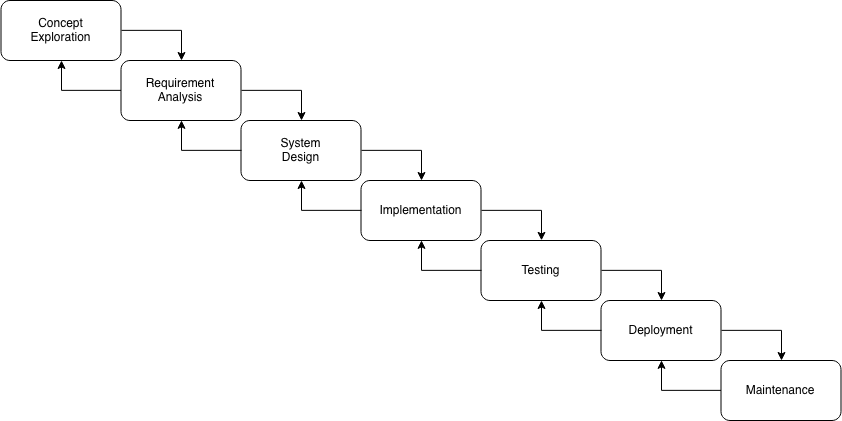
\includegraphics[width=0.69\paperwidth]{./img/waterfall.png}
    \hspace{0.05\linewidth}
    \centering
    \caption{\textit{Waterfall} Model}
		\label{img:waterfall}
    \end{center}
\end{figure}

\section{Implementation Plan}
The Architectural Styles and Patterns of the system to be are huge explained in Section \ref{architecturalStyle}.\\
The implementation of our system will be done module by module and component by component, the most relevant and complex part of the system to be is the \textit{Controller} of the MVC model.\\
The development of the modules must be done keeping attention in writing good \textit{Documentation of the Code}, doing \textit{Unit Test} and
finally making \textit{Code Inspection and Analysis}; these topics are explained in the Section \ref{int_test}.\\
Below there is a Figure in order to explain the implementation flow, several detailed on the \textit{Application Server} components that are the huge part of the \textit{Controller}.

\begin{figure}[H]
  \begin{center}
  	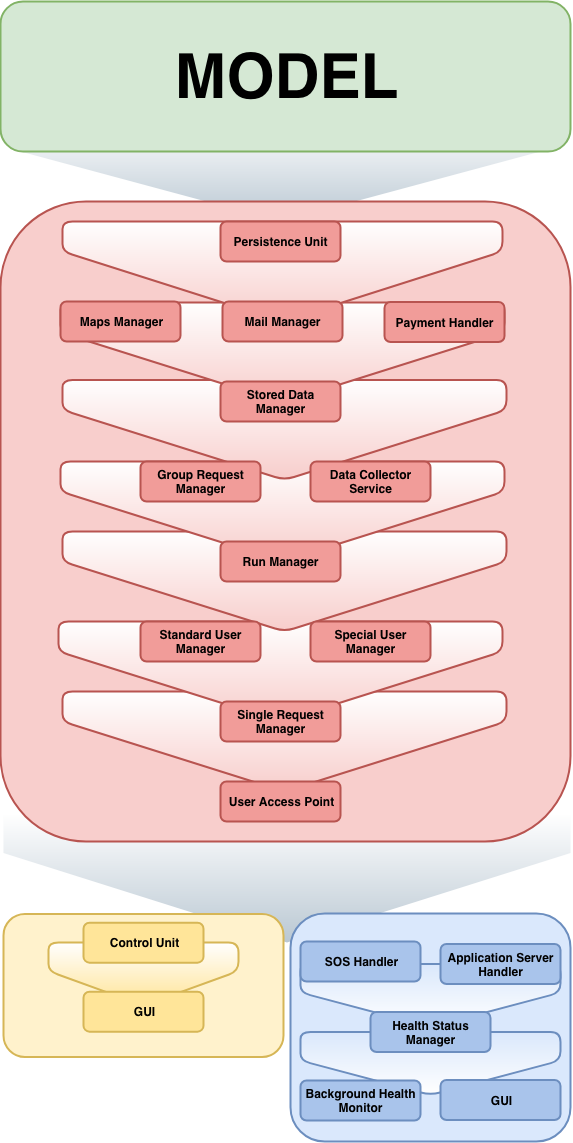
\includegraphics[height=0.59\paperheight]{./img/implementationFlow.png}
    \hspace{0.05\linewidth}
    \centering
    \caption{\textit{Implementation Plan} of the system}
		\label{img:implementationFlow}
    \end{center}
\end{figure}

\subsection{Implementation Plan Discussion}
\myparagraph{}
The \textit{Model} is the first part of the system that must be implemented. This choice is supported by the facts that the \textit{Model} is used by most of the components in the \textit{Application Server} and that some part of it are represented in the \textit{Database}. Moreover, this way it is avoided any type of duplication or confusion between what we consider \textit{Model} and what \textit{Controller}.

\myparagraph{}
The second most relevant part of the system that must be developed is the \textit{Controller}, and we find in it components of the \textit{Application Server}.
\begin{itemize}
  \item \textbf{Persistence Unit} is the first component of this part that must be implemented because it manages all communication with the DBMS and communicates with a large part of the components in this part of the system.
  \item \textbf{Maps Manager}, \textbf{Mail Manger} and \textbf{Payment Handler} are components the provides the majority of services in common among other components and \textit{Maps Manager} and \textit{Payment Handler} are also the components that interfaces with the external services.
  \item \textbf{Group Request Manager} and \textbf{Data Collector Service} provides some of the services provides by \textit{Data4Help}. They are at the base of other components so their implementation must be done keeping attention.
  \item \textbf{Run Manager} is the component that allows our system to manage the \textit{Run}'s services, fault tollerance must be guarantee. It is the core of this service and its implementation is crucial. It also provides an interface to the \textit{Standard User Manager} components and it use the \textit{Maps Manager} component.
  \item \textbf{Standard User Manager} and \textbf{Special User Manager} are the core of all actions performed by a \textit{Generic User} of \textit{Data4Help}. They communicate with most of the components described before and their implementation has to guarantee very high tolerance to fault and good performance since they represent a possible bottleneck of the application.
  \clearpage
  \item \textbf{Single Request Manager} like some previous components it provides one of the core service of \textit{Data4Help}. Its implementation is inserted at this point because it requires some important functionalities of \textit{Standard User Manager} and \textit{Special User Manager}.
\end{itemize}

\myparagraph{}
The \textit{View} is the last part of the system to be that must be implemented because it needs most of the functionalities of the \textit{Controller}.\\
The implementation flow of the internal components of \textit{AutomatedSOS} is specified in Figure \ref{img:implementationFlow} to avoid any possible problems, being a critical service.

\subsection{Implementation Choices}

\subsubsection{Database}
The choices that have been taken for the \textit{Database} are MySQL 5.7 as relational DBMS and InnoDB as Database Engine. This last choice has been taken to manage concurrency while accessing same tables.

\subsubsection{Application Server}
The implementation of this important layer is done with Java Enterprise Edition 7 (JEE) using a GlassFish Server. Java Persistence API (JPA) is used to interface with the DBMS, JAX-RS to implement RESTful APIs to interface with mobile application, \textit{Web Server} and also with the \textit{External Servicies}.

\subsubsection{Mobile App}
The mobile applications must be implemented in two different architecture respecting native languages, Swift for iOS application and Java for Android ones. The communication with the device must be done using the default frameworks of the respective system, moreover the communication with the \textit{Application Server} and \textit{External Services} must be performed with RESTful APIs.

\subsubsection{Web Server}
As we decided to implement the \textit{Application Server} with JEE, that choice is reflected to this layer. We have only to specify that the implementation of the \textit{GUI} must be performed with HTML5 and CSS; \textit{Control Unit} using JavaServer Pages (JSP).

%TODO Implementation Tree

\section{Integration and Testing}\label{int_test}
The Integration and Testing Section provides the main guidelines to explain the integration test phase, describing which tools will be used and planning integration phase in a detailed way.

\subsection{Entry Criteria}
This section describes which are the prerequisites needed before approach the integration phase. We can find three main topics the must be done before starting:
\begin{itemize}
  \item \textbf{Documentation of the Code}: Sometimes the code's documentation is understimate. Good documentation provides tools to review the code and its mean; moreover it is important in huge project, like the \textit{TrackMe} one, where more people will develop the system. It makes easier the understanding of the classes' functionalities and behaviour and it also makes easier their reusing.\\
  Where only text documentation is not sufficient to explain a certain functionality a formal language of specification like JML (Java Modelling Language) is required.
  \item \textbf{Unit Test}: All classes of the project must be tested with Unit Tests that check for each one its behaviour. Unit Test must be done using JUnit tool and line coverage of 90\% is required. Only the \textit{View} part of our project is authorized not to respect the line covarge constraint.
  \item \textbf{Code Inspection and Analysis}: Code Inspection and Analysis is an important phase of the testing part because with an automated tool, such as SonarQube, we can look for code smell and possible bugs of the classes. Solving issues in this phase provides less probability of complex and big problems in the integration phase.
\end{itemize}

\subsection{Elements to be Integrated}
Our system is structured in a multi-tiered client-server architecture and we can divide our system in four main layers (according to Figure \ref{img:layeredStructure}).\\
The integration of the different components in a layer must be done component by component and then when issues of internal integration will be fixed, layers integration that concerns communication between components must be performed.

\subsection{Integration Testing Strategy}
To avoid any possibility of complex problems during the integration phase, it must be performed incrementally, when it is possible, during the growing of the system (As it has been done for the implementation phase).\\
Where integration test is not possible during the developing phase a bottom-up approach of integration must be followed in order to avoid any possible failure of the core components of the system.

\subsection{Integration Sequence}
In this Section the integration flow is explained.\\
Tables will be used to better explain the components that have a role in the integration activity.

\subsubsection{Application Server Components Integration}\label{appServCompIntRef}
Huge part of the integration component/component must be done in the \textit{Application Server} that contains a big part of the \textit{Logic} of the system. The integration must be done keeping attention and avoiding any possible issues.

\begin{center}
\begin{table}[H]
\begin{tabular}{ | l | p{0.4\textwidth} | p{0.4\textwidth} |}
  \hline
    \textbf{\#} & \textbf{Component} & \textbf{Integrated with} \\ \hline
    I01  & Data Collector Service  & Persistence Unit \\ \hline
    I02  & Group Request Manager  & Persistence Unit \\ \hline
    I03  & Group Request Manager  & Payment Handler \\ \hline
    I04  & Run Manager & Persistence Unit \\ \hline
    I05  & Run Manager & Maps Manager \\ \hline
    I06  & Run Manager & Mail Manager \\ \hline
    I07  & Standard User Manager & Persistence Unit \\ \hline
    I08  & Special User Manager & Persistence Unit \\ \hline
    I09  & Standard User Manager & Mail Manager \\ \hline
    I10  & Special User Manager & Mail Manager \\ \hline
    I11  & Standard User Manager & Data Collector Service \\ \hline
    I12  & Special User Manager & Group Request Manager \\ \hline
    I13  & Standard User Manager & Run Manager \\ \hline
    I14  & Single Request Manager & Persistence Unit \\ \hline
    I15  & Single Request Manager & Payment Handler \\ \hline
    I16  & Special User Manager & Single Request Manager \\ \hline
    I17  & Standard User Manager & Single Request Manager \\ \hline
\end{tabular}
\caption{\textit{Application Server} components integration table}
\label{table:appServerIntegrationTable}
\end{table}
\end{center}

\begin{figure}[H]
  \begin{center}
  	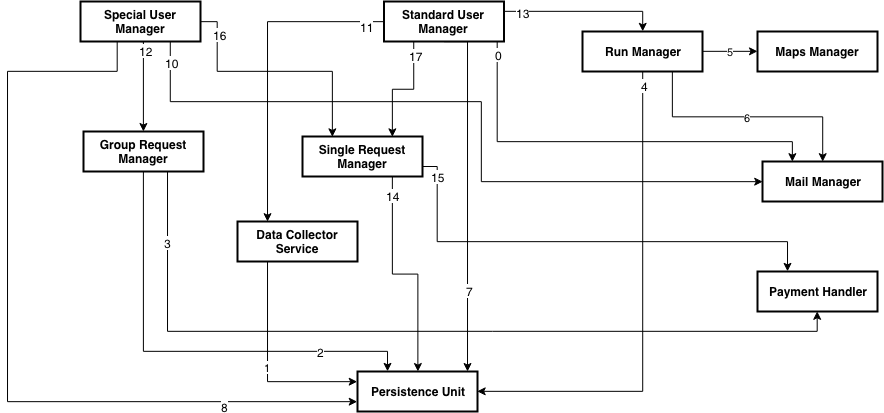
\includegraphics[width=\textwidth]{./img/appServerIntegration.png}
    \hspace{0.05\linewidth}
    \centering
    \caption{\textit{Application Server} components integration diagram}
		\label{img:appServerIntegrationDiagram}
    \end{center}
\end{figure}


\subsubsection{AutomatedSOS Components Integration}
Such as in the \textit{Application Server Components Integration} (Section \ref{appServCompIntRef}) now we want to focus our attention in the integration of \textit{AutomatedSOS} components.

\begin{center}
\begin{table}[H]
\begin{tabular}{ | l | p{0.4\textwidth} | p{0.4\textwidth} |}
  \hline
    \textbf{\#} & \textbf{Component} & \textbf{Integrated with} \\ \hline
    I01  & Health Status Manager  & Application Server Handler \\ \hline
    I02  & Background Health Monitor  & SOS Handler \\ \hline
    I03  & Background Health Monitor  & Health Status Manager \\ \hline
    I04  & GUI  & Application Server Handler \\ \hline
    I05  & GUI & Health Status Manager \\ \hline
\end{tabular}
\caption{\textit{AutomatedSOS} components integration table}
\label{table:automatedIntegrationTable}
\end{table}
\end{center}

\begin{figure}[H]
  \begin{center}
  	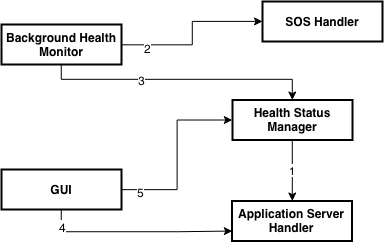
\includegraphics[width=\textwidth]{./img/automatedIntegration.png}
    \hspace{0.05\linewidth}
    \centering
    \caption{\textit{AutomatedSOS} components integration diagram}
		\label{img:automatedIntegrationDiagram}
    \end{center}
\end{figure}

\subsubsection{Subsystems Integration}
Now we present the integration sequence of subsystems. As we mentioned before a bottom-up approach must be followed.

\begin{center}
\begin{table}[H]
\begin{tabular}{ | l | p{0.28\textwidth} | p{0.28\textwidth} | p{0.28\textwidth} |}
  \hline
    \textbf{\#} & \textbf{Subsystems} & \textbf{Component} & \textbf{Integrated with} \\ \hline
    I01 & Database, Application Server & Persistence Unit & DBMS \\ \hline
    I02 & Application Server, External Servicies & Maps Handler & Maps Service \\ \hline
    I03 & Application Server, External Servicies & Payment Hendler & Payment Service \\ \hline
    I04 & Application Server, Web Server & Special User Manager & Control Unit \\ \hline
    I05 & Application Server, Web Server & Standard User Manager & Control Unit \\ \hline
    I06 & Application Server, Web Server & Run Manager & Control Unit \\ \hline
    I07 & Application Server, Mobile Client & Standard User Manager & Application Server Handler \\ \hline
    I08 & Application Server, Mobile Client & Run Manager & Application Server Handler \\ \hline
    I09\textsuperscript{*} & Mobile Client, External Services & SOS Handler & SOS Service \\ \hline
\end{tabular}
\caption{\textit{Subsystems integration} table.
\text{*}:this integration activity is valid only for \textit{AutomatedSOS} application}
\label{table:subsystemsIntegrationTable}
\end{table}
\end{center}

\clearpage

%Effort Spent
\chapter{Effort Spent}
\section{Michele Gatti}

%Space
\smallskip
\begin{center}
\begin{tabular}{ | p{0.75\linewidth} | l | }
  \hline
    \textbf{Task} & \textbf{Hours }\\ \hline
    Purpose and Goals & 1 \\ \hline
    Product Perspective and Product Functions & 6 \\ \hline
    User Characteristics and Constraints & 2 \\ \hline
    Assumptions and Dependencies & 3 \\ \hline
    The World and the Machine & 3 \\ \hline
    Team revision & 1 \\ \hline
    Class Diagram & 6 \\ \hline
    Alloy & 14 \\ \hline
    Team work & 2 \\ \hline
    \textbf{Total} & \textbf{38} \\ \hline
\end{tabular}
\end{center}
%Space
\smallskip


\section{Federica Gianotti}

%Space
\smallskip
\begin{center}
\begin{tabular}{ | p{0.75\linewidth} | l | }
  \hline
    \textbf{Task} & \textbf{Hours }\\ \hline
    Purpose and Goals & 4 \\ \hline
    Scope, Definitions, Acronyms and Abbreviations & 2 \\ \hline
    Team revision & 1 \\ \hline
    Functional Requirements & 14 \\ \hline
    Functional Requirements and Mockup revision & 4 \\ \hline
    Activity Diagrams & 4 \\ \hline
    Class Diagram & 2 \\ \hline
    Alloy & 2 \\ \hline
    Team work & 2 \\ \hline
    Final revision & 3 \\ \hline
    \textbf{Total} & \textbf{38} \\ \hline
\end{tabular}
\end{center}
%Space
\smallskip

\section{Mathyas Giudici}

%Space
\smallskip
\begin{center}
\begin{tabular}{ | p{0.75\linewidth} | l | }
  \hline
    \textbf{Task} & \textbf{Hours }\\ \hline
    \textit{GitHub and LaTeX setup} & \textit{2} \textsuperscript{*} \\ \hline
    Purpose and Goals & 2 \\ \hline
    Scope, Definitions, Acronyms and Abbreviations & 2 \\ \hline
    Team revision & 1 \\ \hline
    Functional Requirements & 14 \\ \hline
    User Interface Mockup & 4 \\ \hline
    Functional Requirements and Mockup revision & 4 \\ \hline
    Activity Diagrams & 3 \\ \hline
    Class Diagram & 2 \\ \hline
    Alloy & 2 \\ \hline
    Team work & 2 \\ \hline
    Final revision & 2 \\ \hline
    \textbf{Total} & \textbf{38} \\ \hline
\end{tabular}
\end{center}

\textsuperscript{*} : GitHub and LaTeX setup hours are not counted in the total of the hours

\clearpage

\clearpage

\appendix
\chapter{Appendix}
\section{Software and Tools}
\begin{itemize}
  \item \text{\LaTeX} used to build this document;
  \item \textit{GitHub} used to manage the different versions of this document;
  \item \textit{draw.io} used to draw diagrams;
  \item \textit{Balsamiq Mockups 3} used to draw mock-ups;
  \item \textit{Alloy Analyzer} used tp analyze our specifications.
\end{itemize}


\section{Changelog}
\begin{itemize}
  \item \textbf{1.0} : First release of this document;
  \item \textbf{2.0} : Corrected \textit{Create a Run} activity diagram;
  \item \textbf{2.0} : Corrected \textit{Fist Individual Log In} and \textit{Change device};
  \item \textbf{2.0} : Corrected \textit{Use Case Diagram};
  \item \textbf{2.0} : Corrected \textit{Reliability requirement};
  \item \textbf{2.0} : Corrected \textit{Class Diagram} and \textit{Alloy}.
\end{itemize}


\begin{thebibliography}{9}

  \bibitem{ieee-29148}
	ISO/IEC/IEEE 29148:2011 \emph{Systems and software engineering - Life cycle processes - Requirements engineering}

  \bibitem{ieee-830}
	IEEE 830:1998 \emph{Recommended Practice for Software Requirements Specifications}

  \bibitem{world-machine}
  M.Jackson \& P. Zave, \emph{The World and The Machine}, 1995

  \bibitem{se-assignments}
  Elisabetta Di Nitto - Software Engineering 2 Slides (AY 2018/2019) \emph{Project goal, schedule and rules}

\end{thebibliography}


\end{document}
